% !Mode:: "TeX:UTF-8"
\documentclass[openright=true,type=master]{hithesis}
% 此处选项中不要有空格
%%%%%%%%%%%%%%%%%%%%%%%%%%%%%%%%%%%%%%%%%%%%%%%%%%%%%%%%%%%%%%%%%%%%%%%%%%%%%%%%
% 必填选项
% type=doctor|master|bachelor
%%%%%%%%%%%%%%%%%%%%%%%%%%%%%%%%%%%%%%%%%%%%%%%%%%%%%%%%%%%%%%%%%%%%%%%%%%%%%%%%
% 选填选项(选填选项的缺省值已经尽可能满足了大多数需求,除非明确知道自己有什么
% 需求)
% glue=true|false
% 	含义:由于我工规范中要求字体行距在一个闭区间内,这个选项为true表示tex自
% 	动选择,为false表示区间内一个最接近版心要求行数的要求的默认值,缺省值为
% 	false。
% tocfour=true|false
% 	含义:是否添加第四级目录,只对本科文科个别要求四级目录有效,缺省值为
% 	false
% fontset=siyuan|windowsnew|windowsold
% 	含义:注意这个选项视为了解决特殊问题而设置,比如用有些发行版本的linux排
% 	版时可能(大多数发行版不会)会遇到的字体无法载入的问题,以及想要解决排
% 	版如biang biang面的biang 这类中易宋体无法识别的汉字的问题。没有特殊的需
% 	要不推荐使用这个选项。
%
%	如果是安装了windowns字体的linux系统,可以填写windowsnew(win vista以后
%	的字体)或windowsold(vista以前)或者想用思源宋体并且是已经安装了思源宋
%	体的任何系统,填写siyuan选项缺省值为空,自动识别系统并匹配字体。模板版
%	中给出的思源字体定义文件定义的思源字体的版本是Adobe版,其他字体是
%	windowsnew字体。
% tocblank=true|false
% 	含义:目录中第一章之前,是否加一行空白。缺省值为true。
% chapterhang=true|false
% 	含义:目录的章标题是否悬挂居中,规范中要求章标题少于15字,所以这个选项
% 	有无没什么用,
%	除了特殊需求。缺省值为true。
% fulltime=true|false
% 	含义:是否全日制,缺省值为true。非全日制如同等学力等,要在cover中设置类
% 	型,封面中不同格式
% subtitle=true|false
% 	含义:论文题目是否含有副标题,缺省值为false,如果有要在cover中设置副标
% 	题内容
% ,封面中显示。
% newgeometry=true|false
% 	含义:规范中的自相矛盾之处,版芯是否包含页眉页脚,旧方法是按照包含页眉
% 	页脚来设置,缺省值为false,即旧方法。
% debug=true|false
% 	含义:是否显示版芯框和行号,用来调试。默认否。
% openright=true|false
% 	含义:博士论文是否要求章节首页在偶数页,此选项不在规范要求中,按个人喜
% 	好自行决定。 默认否。
% caplastcenter=true|false
% 	含义:图题、表题是否居中对齐(我工规范要求居中,但不要求居中对齐),此
% 	选项不在规范要求中,按个人喜好自行决定。默认是。
%%%%%%%%%%%%%%%%%%%%%%%%%%%%%%%%%%%%%%%%%%%%%%%%%%%%%%%%%%%%%%%%%%%%%%%%%%%%%%%%

\usepackage{hithesis}
\graphicspath{{figures/}}

%============================
% 分块矩阵的书写宏包
\usepackage{easybmat}
\usetikzlibrary{patterns}
%============================
\begin{document}

\frontmatter
% !Mode:: "TeX:UTF-8"

\hitsetup{
  %******************************
  % 注意:
  %   1. 配置里面不要出现空行
  %   2. 不需要的配置信息可以删除
  %******************************
  %
  %=====
  % 秘级
  %=====
  statesecrets={公开},
  natclassifiedindex={O332},
  intclassifiedindex={62-1},
  %
  %=========
  % 中文信息
  %=========
%  ctitleone={基于广义线性法的},
%  ctitletwo={结构动响应数值算法设计},
  ctitle={基于广义线性法的结构动响应数值算法设计},
  %csubtitle={一条副标题}, %一般情况没有,可以注释掉
  cxueke={工学},
  csubject={一般力学与力学基础},
  caffil={航天学院\quad 航天工程与力学系},
  cauthor={李金泽},
  csupervisor={于开平教授},
%  cassosupervisor={某某某教授}, % 副指导老师
%  ccosupervisor={某某某教授}, % 联合指导老师
  % 日期自动使用当前时间,若需指定按如下方式修改:
  cdate={\today},
  cstudentid={16S018040},
  cstudenttype={学术型硕士}, %非全日制教育申请学位者
  %(同等学力人员)、(工程硕士)、(工商管理硕士)、
  %(高级管理人员工商管理硕士)、(公共管理硕士)、(中职教师)、(高校教师)等
  %
  %
  %=========
  % 英文信息
  %=========
  etitle={Design of Numerical Algorithms for Structural Dynamcis Based on the General Linear method},
%  esubtitle={This is the sub title},
  exueke={Engineering},
  esubject={General Mechanics},
  eaffil={\emultiline[t]{School of Astronautics}},
  eauthor={Li Jinze},
  esupervisor={Professor Yu Kaiping},
 % eassosupervisor={XXX},
  % 日期自动生成,若需指定按如下方式修改:
  edate={June 2018},
  estudenttype={Master of Science},
  %
  % 关键词用“英文逗号”分割
  ckeywords={\TeX, \LaTeX, CJK, 嗨!, thesis},
  ekeywords={\TeX, \LaTeX, CJK, template, thesis},
}

\begin{cabstract}

摘要的字数(以汉字计),硕士学位论文一般为500 $\sim$ 1000字,博士学位论文为1000 $\sim$ 2000字,
均以能将规定内容阐述清楚为原则,文字要精练,段落衔接要流畅。摘要页不需写出论文题目。
英文摘要与中文摘要的内容应完全一致,在语法、用词上应准确无误,语言简练通顺。
留学生的英文版博士学位论文中应有不少于3000字的“详细中文摘要”。

  关键词是为了文献标引工作、用以表示全文主要内容信息的单词或术语。关键词不超过 5
  个,每个关键词中间用分号分隔。(模板作者注:关键词分隔符不用考虑,模板会自动处
  理。英文关键词同理。)
\end{cabstract}

\begin{eabstract}
   An abstract of a dissertation is a summary and extraction of research work
   and contributions. Included in an abstract should be description of research
   topic and research objective, brief introduction to methodology and research
   process, and summarization of conclusion and contributions of the
   research. An abstract should be characterized by independence and clarity and
   carry identical information with the dissertation. It should be such that the
   general idea and major contributions of the dissertation are conveyed without
   reading the dissertation.

   An abstract should be concise and to the point. It is a misunderstanding to
   make an abstract an outline of the dissertation and words ``the first
   chapter'', ``the second chapter'' and the like should be avoided in the
   abstract.

   Key words are terms used in a dissertation for indexing, reflecting core
   information of the dissertation. An abstract may contain a maximum of 5 key
   words, with semi-colons used in between to separate one another.
\end{eabstract}
 % 封面
\makecover
\begin{denotation}
\begin{table}[h]%此处最好是h
\caption{国际单位制中具有专门名称的导出单位}
\vspace{0.5em}\centering\wuhao
\begin{tabular}{ccccc}
\toprule[1.5pt]
量的名称&单位名称&单位符号&其它表示实例\\
\midrule[1pt]
频率&赫[兹]&Hz&s-1\\
\bottomrule[1.5pt]
\end{tabular}
\end{table}
\end{denotation}
%物理量名称表,符合规范为主,有要求添加
\tableofcontents    % 中文目录
%\tableofengcontents % 英文目录,硕本不要求
%======================================================================
\mainmatter
%\linenumbers debug 选项
%\layout debug 选项
\chapter{绪论}
%
\section{课题来源}
根据导师在研一期间的指导及个人兴趣、基础知识的储备出发,通过查阅相关资料并在导师的指导下共同商定此论文题目。

在大四毕业后的暑假期间根据导师推荐的几篇文章\cite{杨超2015},我开始了学习结构动力学运动方程数值求解算法。同时,在研一上学期由刘伟老师讲解的《高等结构动力学》课程中,我再一次接触到了结构动力学方程的数值求解。同时在该课程实验中,我也第一次发现了满足一些看似可行的直接积分法,求解出的响应有时却并不可靠,例如Wilson-$\theta$法\sindex[china]{Wilson-$\theta$!Wilson-$\theta$}。它的这种特性由于其本身的数值耗散和弥散特性造成的。这次学习让我对求解结构动力学方程的数值算法产生了兴趣。同时,我也知道力学对数学,尤其是计算数学的要求是很高的。于是在研究生期间,又选了很多数学专业的核心课程(非线性数值分析、现代常微分方程理论、小波分析)进行学习,为自己后面进一步的探究数值算法铺平道路。这些数学课程的学习中,我愈发的觉得结构动力学方程的直接积分法的研究还有很多工作可做。特别值得一提就是,似乎在力学中我们更多的是借鉴了线性多步法来发展直接积分法,而使用Runge-Kutta法的思想发展结构动力学求解算法少之甚少。特别就是由Butcher J. C.在1966年提出的更具一般性的算法框架去求解常微分方程\cite{Butcher1966}。在该框架下,线性多步法和Runge-Kutta法都是其特例。这类算法应用到求解结构动力学运动方程还鲜有文献。这也是进行本文研究的一个主要目标。
\section{课题研究背景、目的和意义}
\subsection{结构动响应问题的工程背景}
动力学问题在国民经济和科学技术的发展中有着广泛的应用领域。最常见遇到的是结构动力学问题,它有两类研究对象。一类是在动力状态下工作的机械或结构,例如高速旋转的电机,汽轮机,离心压缩机,冲压机床,以及高速运行的车辆,飞行器等,它们承受本身惯性及与周围介质或结构相互作用的动力载荷。如何保证它们运行的平稳性及结构的安全性,是极为重要的课题。另一类是承受动力载荷作用的工程结构,例如建于地面的高层建筑,反应塔和管道,核电站的安全壳和热交换器。近海工程的海洋石油平台等,他们可能承受强风,水流,地震以及波浪等各种动力载荷的作用。这些结构的破裂、倾覆和垮塌等事故的发生,将给人民的生命财产造成巨大的损失。正确分析和设计这类结构,在理论上和实际上都是具有重要意义的课题。动力学研究的另一重要领域是波在介质中的传播问题。它是研究短暂作用于介质边界或内部的载荷所引起的位移和速度的变化,如何在介质中向周围传播,以及在界面上如何反射,折射等规律。它的研究在结构的抗震设计,人工地震勘测,无损探伤等领域都有广泛的应用背景,因此也是近二十都年一直受到工程和科技界密切关注的课题。
\subsection{结构动响应数值算法的数学力学背景}
一般情况下,大多数工程问题的数学建模后得到的微分方程往往是不可能求出解析解的;或者说,花费很大的努力求得的解析解是不经济的。这也导致了在实际应用中,应用数值算法求解得到的微分方程是一种必要手段。在结构动力学运动方程的求解过程中更是这种情况。

结构动力学数值计算主要有两大类传统方法\cite{于开平2005}。一是在空间域使用有限元离散后,基于大多数工程结构动态响应主要以低频为主的假设,使用模态分解和叠加的步骤,给出模态截断后的动响应,可归类于近似解析法。这类方法适合于比例阻尼假设情况,适合于长时间、持续动载荷作用问题,以及大多数以低频响应为主的工程问题。但对中高频激励问题(基于有限元模型,航天工程更关注的中高频多数指200-2000HZ范围)的计算尚没有很好解决。主要原因是:2000HZ以内可能有很多阶模态,高阶模态对参数变化更为敏感,同时要求更细密的有限元网格\cite{于开平2005}。此外,高阶模态阻尼比的确定也还没有合理的模型,存在精度和计算量两方面的问题。另外一种方法是在时间域使用有限差分,或者使用时间有限元离散,得到时间逐步递推的计算步骤,还有一类是时空域同时离散的时空有限元方法。这类方法属于数值方法,不仅适用于比例阻尼也适用于于非比例阻尼、非线性情况。这类方法也将是本文分析和研究的重点。

目前在大型结构的瞬态动力学、非线性动力学响应数值计算问题上,比较有效的方法仍然是时域内的直接积分方法,又称逐步积分法。该类方法,有合适的精度、合适的计算量以及适合于大多数实际工程问题。也就是说算法数值计算的整体性能好、适用范围广,因此一直受到计算力学、计算数学工作者和工程界的重视。

\subsection{课题研究的意义}
目前,用线性多步法的理论去发展直接积分法的理论比较完善。特别是经过Dahlquist的发展推广\cite{Dahlquist1956},得到了如下结论\cite{book:dover}:
\begin{itemize}
\item[(1)]  一个显式的、A-稳定的线性多步法是不存在的。
\item[(2)]  一个三阶及其以上精度的A-稳定的线性多步法是不存在的。
\item[(3)] 带有最小误差常数的二阶精度的A-稳定的线性多步法是梯形积分规则。
\end{itemize}
于是,想要利用线性多步法的理论去发展具有A-稳定的算法已经是不可能的。然而,在数学分支—常微分方程数值解的理论中,我们也得知通过适当的构造,广义线性法可以突破上述线性多步法的障碍,理论上可以实现任意阶精度下,其数值方法仍能保持一定好的数值特性,例如A-稳定性,甚至L-稳定性。特别地,作为广义线性法的一个特例—Runge-Kutta法,也可以实现上述特性。故本文的研究意义在于,将广义线性法应用到结构动力学运动方程求解中,进而推导出新的求解格式。这些新的算法格式在数学分析框架下具有良好的性质,但应用到力学问题上,可能还需要进行一定的改进和完善。同时,这些新的数值格式也将在力学背景下进行算法的优劣分析,比如,其数值高频耗散、相对周期误差等。特别地,本文也将尝试利用广义线性法中对于非线性常微分方程、刚度问题的分析借鉴到力学中的非线性动力学、刚度硬化问题的分析上。这样可以对现有直接积分法在理论分析非线性问题时,提供一个理论判断依据。
\section{国内外研究现状}
目前,国内外在广义线性法和结构动力学数值算法的发展中,几乎都是相对独立的。鲜有研究者将者二者结合起来。但过去的几十年也有一些研究学者将Runge-Kutta法应用到结构动力学数值求解中,进而构造了一些新的数值算法。

周树荃和高科华\cite{周树荃1992}在论文中利用3级3阶半隐式Runge-Kutta法求解结构动力学问题,并利用多项式预处理共轭梯度法求解有关代数方程组,提出了半隐式RK型并行直接积分法(RK33P).与相应的串行算法RK33S算法进行比较,发现当求解系统的阶数为103-104,其加速度比可达24-27。

Christoph L.和Simeon B.\cite{Lunk2004,Lunk2005}利用Runge-Kutta-Nyström方法求解动力学中的刚性力学系统,该方法一般化了著名的Störmer规则,并且使得求解的稳定域最大化。结果表明,文章提出的RKN方法具有一定的可比性和高效性。

Dopico D.和Lugris U.\cite{Dopico2010}等分析了在实时多体结构系统中具有遗传Runge-Kutta稳定性的广义线性方法(IRK)的两个应用。文章问答了IRK方法是否适合求解实时结构响应以及该类方法是否比传统的Newmark家族方法更优。

吴志桥等人\cite{吴志桥2010}将几种具有不同稳定性的Runge-Kutta方法应用到结构动力学的数值求解中,并且使用了减小计算量的两种方法:使用单对角隐式Runge-Kutta方法和应用转化矩阵,算例表明在精确解上较小的物理阻尼能有效抑制高频分量,但对各种直接积分方法的影响较小,较高精度的L-稳定Runge-Kutta方法能有效抑制高频分量的同时高精度的求解低频振动。而且在他的博士论文\cite{吴志桥2009}中,通过研究Runge-Kutta方法对结构动力学运动方程的求解格式,得到A-稳定与直接积分法中的无条件稳定是等价的,而L-稳定格式包含数值阻尼。

Yin S. H.\cite{Yin2013}通过在结构动力学数值求解格式中构造位移和速度显式更新公式,推导出带四个参数的放大矩阵,同时利用Runge-Kutta方法求解对应的结构动力学运动微分方程得到其状态向量的迭代格式,进而得到其迭代矩阵,最后通过让放大矩阵和迭代矩阵对应风量相等,得到其位移速度更新公式中的四个参数,结果表明其参数是结构依赖的。

郭静和邢誉峰\cite{郭静2014}在2014年利用2级4阶隐式Guass-Lengendre辛Runge-Kutta方法(GLSRK)求解有阻尼和外荷载情况下的线性动力学运动方程。并首次给出了Guass-Lengendre辛RK方法和经典RK方法的谱半径和单步相位误差的显式表达式。通过算例表明,辛RK方法比经典RK方法优越,尤其是在运动学特性和长时间数值模拟方面尤为显著;但是该算法与传统的Newmark-$\beta$法相比,计算量和储存量过于庞大,这也在一定程度上限制了该方法的应用。

针对上述问题,黄策、富明慧\cite{黄策2016}等人将郭静等人提出的四阶隐式Guass-Lengendre辛RK法进行优化,先通过消元,降低问题的规模,再利用消元后得到的方程系数矩阵正定对称的特点,采用预处理共轭梯度法求解。与原算法相比,改进后的算法大幅度降低了储存量和计算量;同时与Newmark-$\beta$法相比,在未明显增加计算量的前提下,大幅度提高了计算精度。

可以看出,国内外利用Runge-Kutta方法去求解结构动力学方程的研究也是较为零散的,还有大量的工作可做。
\section{本文主要研究内容}
本文将从数学常微分方程数值方法—广义线性法和力学中结构动力学运动方程的结构依赖型直接积分法两个角度出发,针对动力学运动方程的数值解法进行探究。本论文的主要研究内容有:
\begin{itemize}
\item 系统学习和探究广义线性法的体系框架。总结广义线性法至今为止的研究成果和应用领域。同时,以广义线性法的知识框架去进一步学习和研究线性多步法。
\item 对现阶段新兴的的结构依赖型算法进一步系统研究。挖掘新的具有实用价值的算法。同时对利用其它构造思想去发展结构动力学数值解法的文献进行总结和归纳。
\item 将广义线性法的几类主要分支算法进行研究,并尝试将其应用到结构动力学数值求解中,以期望获得很好的数值算法。目前根据现有文献研究表明,这种思路是可行的,但可能需要做进一步的细致工作研究。
\item 将广义线性法对非线性系统的刻画应用到直接积分法求解结构动力学非线性系统的分析。
\item 将上述发展算法进行C++或MATLAB代码实现,得到其相应的工具包。
\end{itemize}
%
\chapter{积分算法的设计及基本分析}
对于结构动力学运动方程
\begin{equation}
M\ddot{U}(t)+C\dot{U}(t)+KU(t)=F(t)\label{eq:ch2DyEq}
\end{equation}
的数值求解及其数值算法的设计分析,许多的基本概念借助于数学上对一阶微分方程
\begin{equation}
\dot{y}(t)=f(y,t)\label{eq:ch2Firsty}
\end{equation}
的数值算法的设计分析,如数值算法的相容性、稳定性和收敛性等。事实上,结构动力学运动方程(\ref{eq:ch2DyEq})本质上就是一个二阶的线性微分方程,通过引入速度为独立的变量,可以将其二阶微分形式降维为具有形如(\ref{eq:ch2Firsty})形式的更高阶一阶微分方程。因此,在这一节主要针对(\ref{eq:ch2Firsty})进行数值算法性能指标分析,如果一些定义对于二阶微分方程有差异,再具体指出。

由于广义线性法是求解微分方程(\ref{eq:ch2Firsty})更具一般性的方法,因此本节先通过最简单的数值算法(Euler法)分析引出广义线性法,而后后续的算法性能分析都尽可能在广义线性的基础上进行定义及分析。而常见的线性多步法和Runge-Kutta法将是由其特例导出。

\section{广义线性法}
在20世纪初.Euler在他的著作中,针对如下自治的一阶微分方程
\begin{equation}
\dot{y}(t)=f(y(x))\label{eq:ch2FirstAuto}
\end{equation}
带有合适的初始条件$y(x_0)=y_0\in\mathbf{X}$的数值求解,给出了如下的数值格式
\begin{equation}
y_n=y_{n-1}+h_nf(y_{n-1}),\qquad n=1,2,\cdots\label{eq:ch2Euler}
\end{equation}
对于每一个给定的$n$值,其$y_n$都可以根据上式由$y_{n-1}$计算得到。同时,$h_n$为在第$n$的积分步长,一般情况下没必要要求在整个积分过程中相等,亦即变时间步长积分。但在本文整个分析过程中,我们假定其数值算法都是在相等的时间步长内进行积分及计算的。亦即
\begin{equation}
h_n\equiv h\qquad n=1,2,\cdots
\end{equation}

显然,该数值格式的优劣很大程度依赖于积分步长$h$以及等式(\ref{eq:ch2FirstAuto})右端项$f(y)$随变量$y$的变化快慢程度。而后者通常由$f(y)$满足的Lipschitz常数$L$来度量。同时,我们也需要提及该条件也保证了微分方程(\ref{eq:ch2FirstAuto})解的存在唯一性。于是,我们在本全文中都假定分析的微分方程都满足该Lipschitz条件。关于该条件的对其微分方程解的存在唯一性的证明,读者可以翻阅任意一本常微分方程的书籍都可以查到。这里不再做过多累述。

事实上,Euler格式(\ref{eq:ch2Euler})简单易用,但它却是条件稳定的且只有一阶精度。在很多时候,并不是很实用。因此,后续许多学者提出了很多改进Euler格式的算法。其中,至少有两个策略进行改进Euler方法
\begin{itemize}
\item[\ddag] 单步内使用更多、更复杂的计算,如Runge-Kutta法。
\item[\ddag] 使用更多已知节点的逼近值。如线性多步法。
\item[\ddag] 更高阶导数值的使用。如Rosenbrock方法。
\item[\ddag] 多步-多级-多导数方法。如拟Runge-Kutta方法。
\end{itemize}

从简单的Euler格式出发,我们可以建立如图\ref{Fig:ch2GeneraAxis}的改进策略坐标系
\begin{figure}[htpb]
\centering
\begin{tikzpicture}[xscale=1.2,yscale=1.2]
\draw [thin,->] (0,0) -- (2,1) node [align=center,below right] {每步更多的\\ 计算量};
\draw [thin,->] (0,0)--(-2,1.5) node [align=center,below left] {更多的\\ 已知节点值};
\draw [thin,->] (0,0)--(0,2) node [left] {$y$的导数};
\draw [thin,->] (0,2) -- (0,4) node [left] {$f$的导数};
%============================================
\draw [thin,fill,red] (0,0) circle [radius = 0.03] node [below] {Euler格式};
\end{tikzpicture}
\bicaption[Fig:ch2GeneraAxis]{}{Euler格式的改进策略示意图}{Fig.$\!$}{Generalizations of the Euler method}
\end{figure}

在图\ref{Fig:ch2GeneraAxis}的坐标系下,现阶段的大多数的数值算法都可以被建立在这个三维算法格式空间中,如图\ref{Fig:ch2GeneraEuler}所示。
\begin{figure}[htpb]
\centering
\begin{tikzpicture}[xscale=1.2,yscale=1.2]
\draw [thin] (0,0) -- (2.5,1) node [right] {Runge-Kutta法};
\draw [thin] (0,0)--(-2,1.5) node [left] {线性多步法};
\draw [thin,dashed] (-2,1.5)--(0.5,2.5);
\draw [thin,dashed] (2.5,1) -- (0.5,2.5);
%============================================
\draw [thin] (0,3) node [left] {泰勒级数法} -- (2.5,4);
\draw [thin] (0,3)--(-2,4.5) node [left] {Obreshkov方法};
\draw [thin,dashed] (-2,4.5)--(0.5,5.5);
\draw [thin,dashed] (2.5,4) -- (0.5,5.5);
%--------------------------------
\draw [thin] (0,3) -- (0,0);
\draw [thin] (2.5,4) -- (2.5,1);
\draw [thin] (-2,4.5) -- (-2,1.5);
\draw [thin,dashed] (0.5,2.5) -- (0.5,5.5);
%=-==========================================
\draw [thin] (0,6) -- (2.5,7) node [right] {Rosenbrock方法};
\draw [thin] (0,6)--(-2,7.5);
\draw [thin] (-2,7.5)--(0.5,8.5);
\draw [thin] (2.5,7) -- (0.5,8.5);
%--------------------------------
\draw [thin] (0,6) -- (0,3);
\draw [thin] (2.5,7) -- (2.5,4);
\draw [thin] (-2,7.5) -- (-2,4.5);
\draw [thin,dashed] (0.5,5.5) -- (0.5,8.5);
%=-==========================================
\draw [thin,fill,red] (0,0) circle [radius = 0.03] node [below] {Euler格式};
\draw [thin,fill,blue] (0.5,2.5) circle [radius = 0.03] node [right] {广义线性法};
\draw [thin,fill] (0,3) circle [radius = 0.03];
\draw [thin,fill] (2.5,7) circle [radius = 0.03];
\draw [thin,fill] (-2,4.5) circle [radius = 0.03];
\draw [thin,fill] (2.5,1) circle [radius = 0.03];
\draw [thin,fill] (-2,1.5) circle [radius = 0.03];
\end{tikzpicture}
\bicaption[Fig:ch2GeneraEuler]{}{Euler格式的改进算法框架}{Fig.$\!$}{Generalized formworks of the Euler method}
\end{figure}
于是,可以知道广义线性法是线性多步法和Runge-Kutta法的结合,更是Euler格式的一般化推广。同时,从该图可以知道,广义线性法并不能包括所有的数值格式,它仅仅是现阶段数值算法的一大类。

广义线性方法即结合了线性多步法的多值特点,又使用了Runge-Kutta方法的多级属性。并且它首次由Butcher教授在1966年提出\cite{Butcher1966}。下面提及的广义线性法的矩阵表示形式则是由Burrage和Butcher在1980年引入而来\cite{Burrage1980}。

假定在单步内进行转换的量有$r$个。在第$n$步的开始,这$r$个量被表示为$y_1^{[n-1]},y_2^{[n-1]},\cdots,y_r^{[n-1]}$。当第$n$步完成计算时,对应的$r$量分别为$y_1^{[n]},y_2^{[n]},\cdots,y_r^{[n]}$,并且这些量将作为下一个时间步内的起始值进行后续计算。同时,在单步内计算的$s$个级数值$Y_1,Y_2,\cdots,Y_s$所对应的级数导数值为$F_1,F_2,\cdots,F_S$。为了表示方便,引入如下的$r$或$s$维向量表示,即
\begin{equation}
y^{[n-1]}=\begin{bmatrix}
y_1^{[n-1]}\\
y_2^{[n-1]}\\
\vdots\\
y_r^{[n-1]}
\end{bmatrix},\quad
y^{[n]}=\begin{bmatrix}
y_1^{[n]}\\
y_2^{[n]}\\
\vdots\\
y_r^{[n]}
\end{bmatrix},\quad
Y^{[n]}=\begin{bmatrix}
Y_1^{[n]}\\
Y_2^{[n]}\\
\vdots\\
Y_s^{[n]}
\end{bmatrix},\quad
F(Y^{[n]})=\begin{bmatrix}
f(Y_1^{[n]})\\
f(Y_2^{[n]})\\
\vdots\\
f(Y_s^{[n]})
\end{bmatrix}
\end{equation}

类似于Runge-Kutta方法,级数值$Y_i$是依赖于级数导数值$F_i$的线性组合来计算,但是现在的广义线性法将其推广为不仅依赖于级数导数值的线性组合,也依赖于前述已知节点逼近值$y_i$的线性组合。即
\begin{equation}
Y_i=\sum_{j=1}^{s}ha_{ij}f(Y_j^{[n]})+\sum_{j=1}^{r}u_{ij}y_j^{[n-1]},\qquad i=1,2,\cdots,s
\end{equation}
同理,对于输出量$y_i^{[n]}$也是不仅线性依赖于各个级数导数值$F_i=f(Y_i)$而且也是线性依赖于前述已知节点逼近值$y_i$,即
\begin{equation}
y_i^{[n]}=\sum_{j=1}^{s}hb_{ij}f(Y_j^{[n]})+\sum_{j=1}^{r}v_{ij}y_j^{[n-1]},\qquad i=1,2,\cdots,r
\end{equation}

令$A=[a_{ij}]_{s\times s},U=[u_{ij}]_{s\times r},B=[b_{ij}]_{r\times s}$以及$V=[v_{ij}]_{r\times r}$,同时使用Kronecker积符号($\otimes$),广义线性法则可以表示为
\begin{align}
Y^{[n]}&=h(A\otimes I)F(Y^{[n]})+(U\otimes I)y^{[n-1]}\\
y^{[n]}&=h(B\otimes I)F(Y^{[n]})+(V\otimes I)y^{[n-1]}
\end{align}
其中,$I$表示维度相容的单位矩阵。而Kronecker积定义如下
\begin{equation}
A\otimes I=\begin{bmatrix}
a_{11} I&&a_{12}I&&\cdots && a_{1s} I\\
a_{21}I&&a_{22}I&&\cdots && a_{2s}I\\
\vdots &&\vdots && &&\vdots\\
a_{s1}I &&a_{s2}I&&\cdots &&a_{ss}I
\end{bmatrix}
\end{equation}
进一步,广义线性法可以被表达为如下形式
\begin{equation}
\begin{bmatrix}
\begin{array}{c}
Y^{[n]}\\ \hline
y^{[n]}
\end{array}
\end{bmatrix}=\begin{bmatrix}
\begin{array}{c|c}
A\otimes I & U\otimes I \\ \hline
B\otimes I & V\otimes I
\end{array}
\end{bmatrix}\begin{bmatrix}
\begin{array}{c}
hF(Y^{[n]})\\ \hline
y^{[n-1]}
\end{array}
\end{bmatrix}
\end{equation}

通常情况下,广义线性法的数值性能就被这四个矩阵所决定,即$A,U,B$和$V$。因此对于一个广义线性法,可以用如下的分块矩阵刻画
\begin{equation}
\begin{bmatrix}
\begin{BMAT}[5pt]{c:c}{c:c}
	A & U \\
	B & V
\end{BMAT}
\end{bmatrix}
\end{equation}

当四个矩阵取值不同时,对应着不同的广义线性法。特别地,线性多步法和Runge-Kutta都是其特例。
\subsection{线性多步法}
考虑对于一阶微分方程(\ref{eq:ch2Firsty})的$k$步线性多步法
\begin{equation}
y_n=\sum_{j=1}^{k}\alpha_jy_{n-j}+h\sum_{j=0}^{k}\beta_jf(y_{n-j})\label{eq:ch2lms}
\end{equation}
令$Y^{[n]}=y_n$,并且
\begin{subequations}
\begin{align}
y^{[n]}&=[y_n,y_{n-1},\cdots,y_{n-k+1},hf(y_n),hf(y_{n-1}),\cdots,hf(y_{n-k+1})]^{\text{T}}\\
y^{[n-1]}&=[y_{n-1},y_{n-2},\cdots,y_{n-k},hf(y_{n-1}),hf(y_{n-2}),\cdots,hf(y_{n-k})]^{\text{T}}
\end{align}
\end{subequations}
于是,对于$k$步的线性多步法(\ref{eq:ch2lms})可以写成广义线性法的形式\cite{Burrage1980},即$r=2k,s=1$
\begin{equation}
\begin{bmatrix}
\begin{BMAT}[5pt]{c:c}{c:c}
A & U\\
B & V
\end{BMAT}
\end{bmatrix}=\begin{bmatrix}
\begin{BMAT}[5pt]{c:cccccccc}{c:cccccccc}
\beta_0 & \alpha_1 & \cdots & \alpha_{k-1} & \alpha_k & \beta_1 & \cdots & \beta_{k-1} & \beta_k\\
\beta_0 & \alpha_1 & \cdots & \alpha_{k-1} & \alpha_k & \beta_1 & \cdots & \beta_{k-1} & \beta_k\\
0 & 1 & \cdots & 0 & 0 & 0 & \cdots & 0 & 0\\
\vdots & \vdots & \ddots &\vdots & \vdots &\vdots &\ddots &\vdots &\vdots \\
0 & 0 &\cdots & 1 & 0 &0 &\cdots & 0 & 0 \\
1 & 0 & \cdots & 0 & 0 & 0 & \cdots & 0 & 0\\
0 & 0 & \cdots & 0 & 0 & 1 & \cdots & 0 & 0\\
\vdots & \vdots & \ddots &\vdots & \vdots &\vdots &\ddots &\vdots &\vdots \\
0 & 0 & \cdots & 0 & 0 & 0 & \cdots & 1 & 0
\end{BMAT}
\end{bmatrix}
\end{equation}
特别地,$k$步的线性多步法(\ref{eq:ch2lms})也可以写成$r=k,s=1$的广义线性法形式\cite{Butcher2006c}。文\inlinecite{Butcher2006c}中定义
\begin{equation}
y_i^{[n-1]}=\sum_{j=k-i+1}^{k}(\alpha_jy_{n+k-i-j}+h\beta_jf(y_{n+k-i-j})),\quad i=1,2,\cdots,k\label{eq:ch2skeel}
\end{equation}
其实,公式(\ref{eq:ch2skeel})在文献\inlinecite{Skeel1979}就已经被提出来了,只不过没有涉及广义线性法的应用。于是,线性多步法(\ref{eq:ch2lms})则可以写成如下形式
\begin{equation}
y_n=h\beta_0f(y_n)+\sum_{j=1}^{k}(\alpha_jy_{n-j}+h\beta_jf(y_{n-j}))=h\beta_0f(y_n)+y_k^{[n-1]}
\end{equation}
进一步,在$n$步结束时有
\begin{equation}
\begin{aligned}
y_i^{[n]}&=\sum_{j=k-i+1}^{k}(\alpha_jy_{n+1+k-i-j}+h\beta_jf(y_{n+1+k-i-j}))\\
&=\alpha_{k-i+1}y_n+h\beta_{k-i+1}f(y_n)+\sum_{j=k-i+2}^{k}(\alpha_jy_{n+1+k-i-j}+h\beta_jf(y_{n+1+k-i-j}))\\
&=(\alpha_{k-i+1}\beta_0+\beta_{k-i+1})hf(y_n)+\alpha_{k-i+1}y_k^{[n-1]}+y_{i-1}^{[n-1]}
\end{aligned}
\end{equation}
其中,$i=1,2,\cdots,k$。线性多步法(\ref{eq:ch2lms})的另外一种广义线性法的表出形式为
\begin{equation}\displaystyle
\begin{bmatrix}
\begin{BMAT}[5pt]{c:c}{c:c}
A & U\\
B & V
\end{BMAT}
\end{bmatrix}=\begin{bmatrix}
\begin{BMAT}[5pt]{c:cccccc}{c:cccccc}
\beta_0 & 0 & 0 & 0 & \cdots & 0 & 1\\
\alpha_k\beta_0+\beta_k & 0 & 0 & 0 & \cdots & 0 & \alpha_k\\
\alpha_{k-1}\beta_0+\beta_{k-1} & 1 & 0 & 0 & \cdots & 0 & \alpha_{k-1}\\
\alpha_{k-2}\beta_0+\beta_{k-2} & 0 & 1 & 0 & \cdots & 0 & \alpha_{k-2}\\
\vdots & \vdots & \vdots & \vdots & \ddots & \vdots & \vdots \\
\alpha_{2}\beta_0+\beta_{2} & 0 & 0 & 0 & \cdots & 0 & \alpha_{2}\\
\alpha_{1}\beta_0+\beta_{1} & 0 & 0 & 0 & \cdots & 1 & \alpha_{1}\\
\end{BMAT}
\end{bmatrix}
\end{equation}
其中,$Y^{[n]}=y_n$,而$y^{[n]}$则为
\begin{equation}
y^{[n]}=[y_1^{[n]},y_2^{[n]},\cdots,y_{k-1}^{[n]},y_{k}^{[n]}]^{\text{T}}
\end{equation}
\subsubsection{Adams算法}
线性多步法中,求解非刚性问题时最常用的方法就是Adams方法族。对于线性多步法公式(\ref{eq:ch2lms})中,令
\begin{equation}
\alpha_1=1,\qquad \alpha_i=0,\ i>1
\end{equation}
于是,Adams算法的一般形式为
\begin{equation}
y_n=y_{n-1}+h\sum_{j=0}^{k}\beta_jf(y_{n-j})\label{eq:ch2Adams}
\end{equation}
需要说明的是,算法(\ref{eq:ch2Adams})的显式形式通常称为Adams-Bashforth算法;而其隐式算法则称为Adams-Moulton算法。

于是将Adams算法改写成广义线性法的形式,则有
\begin{equation}
\begin{bmatrix}
\begin{BMAT}[4.5pt]{c}{c:cccccc}
Y_1\\
y_n\\
hf(y_n)\\
hf(y_{n-1})\\
hf(y_{n-2})\\
\vdots\\
hf(y_{n-k+1})
\end{BMAT}
\end{bmatrix}=\begin{bmatrix}
\begin{BMAT}[5pt]{c:cccccc}{c:cccccc}
\beta_0 & 1 & \beta_1 & \beta_2 & \cdots & \beta_{k-1} & \beta_k\\
\beta_0 & 1 & \beta_1 & \beta_2 & \cdots & \beta_{k-1} & \beta_k\\ 
1		& 0 & 0		  & 0   &\cdots &0 &0\\
0		& 0 & 1		  & 0   &\cdots &0 &0\\
0		& 0 & 0		  & 1   &\cdots &0 &0\\
\vdots & \vdots & \vdots & \vdots & \ddots & \vdots & \vdots\\
0	& 0 & 0		  & 0   &\cdots &1 &0
\end{BMAT}
\end{bmatrix}\begin{bmatrix}
\begin{BMAT}[4.5pt]{c}{c:cccccc}
hf(Y_1)\\
y_{n-1}\\
hf(y_{n-1})\\
hf(y_{n-2})\\
hf(y_{n-3})\\
\vdots\\
hf(y_{n-k})
\end{BMAT}
\end{bmatrix}
\end{equation}

尽管Adams-Moulton算法是隐式的,由于其较小的稳定域,它们也仅仅只在求解非刚性问题时使用。除此之外,它们也常常在作为预测-校正格式使用。
\subsubsection{预测-校正格式}
预测-校正格式中,使用Adams-Bashforth方法作为一个预测逼近算法,而Adams-Moulton作为校正格式算法。同时,预测-校正格式通常简写为“PEC”或者“PECE”,其中“P”代表预测格式,而“E”表示计算,“C”表示校正格式。其算法一般形式可写为
\begin{subequations}
\begin{align}
y_n^*&=y_{n-1}+h\sum_{j=1}^{k}\beta_j^*f(y_{n-j})\\
y_n&=y_{n-1}+h\beta_0f(y_n^*)+h\sum_{j=1}^{k}\beta_jf(y_{n-j})
\end{align}
\end{subequations}




















\section{相容性}

\section{稳定性}

\section{收敛性}

\section{精度分析}

\subsection{数值耗散}

\subsection{数值弥散}

\section{超调行为}

\section{虚假根分析}

\section{直接积分法的放大矩阵}

\begin{definition}
直接积分算法的一致性\cite{Hoff1988}。如果两个直接积分算法的放大矩阵$A$的对应元素分别相等\footnote{这也是矩阵相等的定义。},则称这两个积分算法是一致的。
\end{definition}

\begin{definition}
直接积分算法的相似性/谱等价\cite{Hoff1988}。如果两个直接积分算法的放大矩阵$A$的不变量分别对应相等,则称这两个积分算法是相似的/谱等价的。
\end{definition}

需要说明的是,一般情况下,两个谱等价的算法并不一定能导出一致的数值算法特性;而两个算法的一致性可以保证。这样的例子可以参见文献\inlinecite{Hoff198887}。

\section{本章小结}



%
\chapter{结构动响应数值算法研究现状}


\section{传统直接积分法}



\section{结构依赖型直接积分法}



\section{复合型子步隐式算法}
Tarnow和Simo\inlinecite{Tarnow1994}在1994年提出了一个子步复合方法,将一般的二阶直接积分法的精度提高到四阶。在该方法中,一个时间步长内需要三次的子步计算。同时原来的二阶方法的稳定、守恒性质仍保持不变。需要注意的是,当该方法运用到二阶的Newmark-$\beta$方法\cite{Newmark1959}时,导出的高阶算法是没有数值耗散的。为了引入高频耗散特性,需要对求得的响应进行一定的技术处理,如后处理的滤波技术\cite{Fung1998}。后来,又有许多研究学者进行进一步的探索,发展了许多可靠优质的直接积分算法。其中,麻省理工的K.J. Bathe教授在2005年提出了一个两子步算法\cite{Bathe2005,Bathe2007,Bathe2012a}。假设在$t$时刻的状态量,即$^{t}U,^{t}\dot{U},^{t}\ddot{U}$,都是已知的。为了求在时刻$t+\Delta t$的未知量$^{t+\Delta t}U,^{t+\Delta t}\dot{U},^{t+\Delta t}\ddot{U}$,该方法将一个时间步长$\Delta t$划分为两个子时间步长$\gamma\Delta t,(1-\gamma)\Delta t$。在前一个时间子步$\gamma\Delta t$内,采用Trapezoidal规则\cite{book:dover}进行计算,即
\begin{align}
^{t+\gamma\Delta t}\dot{U}&=^{t}\dot{U}+\frac{^t\ddot{U}+^{t+\gamma\Delta t}\ddot{U}}{2}\gamma\Delta t\\
^{t+\gamma\Delta t}{U}&=^{t}U+\frac{^t\dot{U}+^{t+\gamma\Delta t}\dot{U}}{2}\gamma\Delta t
\end{align}




\section{本章小结}

%
\chapter{基于广义线性法的结构动响应数值算法设计}


\section{本章小结}%
\chapter{数值算例}

\section{本章小结}
%
%% !Mode:: "TeX:UTF-8" 

\chapter{示例文档}[Example]

这是 \hithesis\ 的示例文档,基本上覆盖了模板中所有格式的设置。建议大家在使用模板
之前,除了阅读《\hithesis\ 用户手册》,这个示例文档也最好能看一看。
这个示例文档尽量使用到所有的排版格式,然而对于一些不在我工规范中规定的文档,理论
上是由用户自由发挥,这里不给出样例。需要另行载入的宏包和自定义命令在文件
`hithesis.sty'中有示例,这里不列举。

\section{索引示例}[Index]

为便于检索文中内容,可编制索引置于论文之后(根据需要决定是否设置)。索引以论文中
的专业词语为检索线索,指出其相关内容的所在页码。索引用中、英两种文字书写,中文在
前。\sindex[china]{qi!乔峰}\sindex[english]{Xu Zhu}\sindex[english]{Qiao Feng}
中文按各词汉语拼音第一个字母排序,英文按该词第一个英文字母排序。

\section{引用}[Cite]

\sindex[china]{du!段誉}引文标注遵照GB/T7714-2005,采用顺序编码制。正文中引用文献的标示应置于所引内容最后一个字的右上角,所引文献编号用阿拉伯数字置于方括号“[ ]”中,用小4号字体的上角标。要求:

(1)引用单篇文献时,如“二次铣削\cite{cnproceed}”。

(2)同一处引用多篇文献时,各篇文献的序号在方括号内全部列出,各序号间用“,”,如
遇连续序号,可标注讫序号。如,…形成了多种数学模型\cite{cnarticle,cnproceed}…

(3)多次引用同一文献时,在文献序号的“[ ]”后标注引文页码。如,…间质细胞CAMP含量
测定\cite[100-197]{cnarticle}…。…含量测定方法规定
\cite[92]{cnarticle}…。

(4)当提及的参考文献为文中直接说明时,则用小4号字与正文排齐,如“由文献\inlinecite{hithesis2017}可知”

\section{图片}[Pictures]
图应有自明性。插图应与文字紧密配合,文图相符,内容正确。选图要力求精练,插图、照
片应完整清晰。机械工程图:采用第一角投影法,严格按照GB4457~GB131-83《机械制图》
标准规定。数据流程图、程序流程图、系统流程图等按GB1526-89标准规定。电气图:图形
符号、文字符号等应符合附录3所列有关标准的规定。流程图:必须采用结构化程序并正确
运用流程框图。对无规定符号的图形应采用该行业的常用画法。坐标图的坐标线均用细实线
,粗细不得超过图中曲线;有数字标注的坐标图,必须注明坐标单位。照片图要求主题和主
要显示部分的轮廓鲜明,便于制版。如用放大或缩小的复制品,必须清晰,反差适中。照片
上应有表示目的物尺寸的标度。引用文献中的图时,除在正文文字中标注参考文献序号以外
,还必须在中、英文表题的右上角标注参考文献序号。

\subsection{博士毕业论文双语题注}[Doctoral picture example]
\begin{figure}[htpb]
\centering
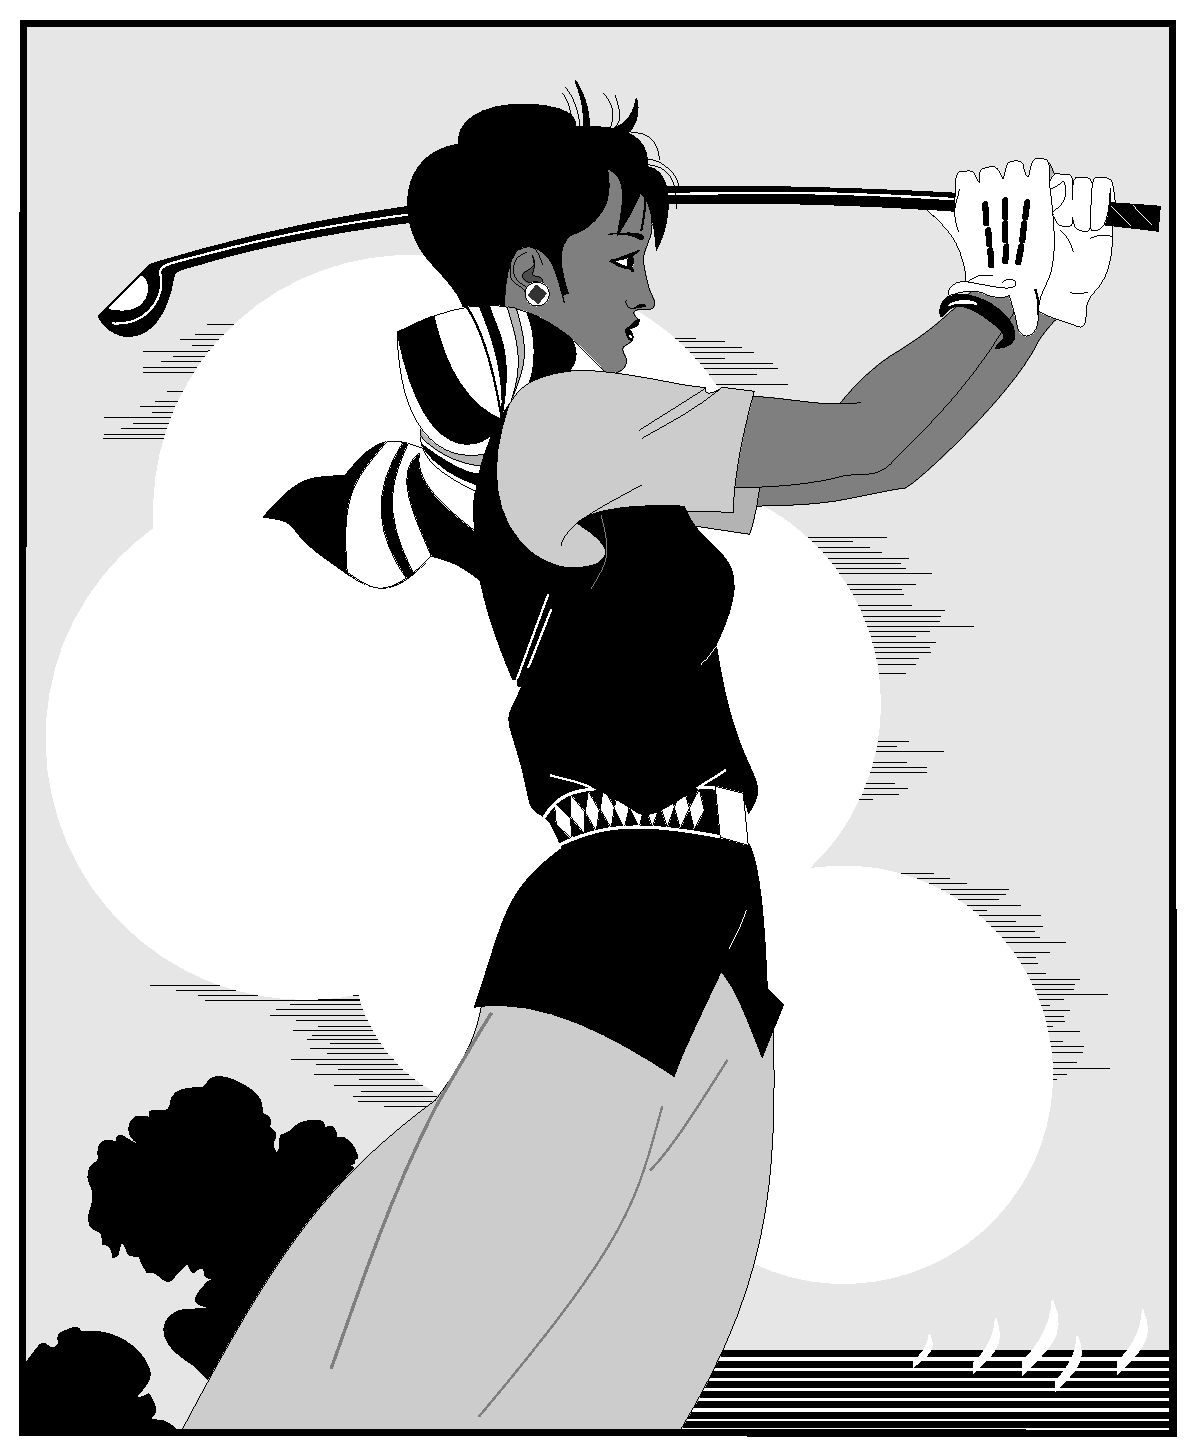
\includegraphics[width = 0.4\textwidth]{golfer}
\bicaption[golfer1]{}{图打打高尔夫球的人打高尔夫球的人打高尔夫球的人打高尔夫球球的人高尔夫球的人球的人高尔夫球的人的人高尔夫球的人}{Fig.$\!$}{The person playing golf playing golf playing golf playing golf playing golf playing golf playing golf playing golf}
\end{figure}

每个图均应有图题(由图序和图名组成),图题不宜有标点符号,图名在图序之后空1个半
角字符排写。图序按章编排,如第1章第一个插图的图号为“图1-1”。图题置于图下,硕士论
文只用中文,博士论文用中、英两种文字,居中书写,中文在上,要求中文用宋体5号字,
英文用Times New Roman 5号字。有图注或其它说明时应置于图题之上。引用图应注明出处
,在图题右上角加引用文献号。图中若有分图时,分图题置于分图之下或图题之下,可以只
用中文书写,分图号用a)、b)等表示。图中各部分说明应采用中文(引用的外文图除外)或
数字符号,各项文字说明置于图题之上(有分图时,置于分图题之上)。图中文字用宋体、
Times New Roman字体,字号尽量采用5号字(当字数较多时可用小5号字,以清晰表达为原
则,但在一个插图内字号要统一)。同一图内使用文字应统一。图表中物理量、符号用斜体
。
\subsection{本硕论文题注}[Other picture example]
\begin{figure}[h]
\centering
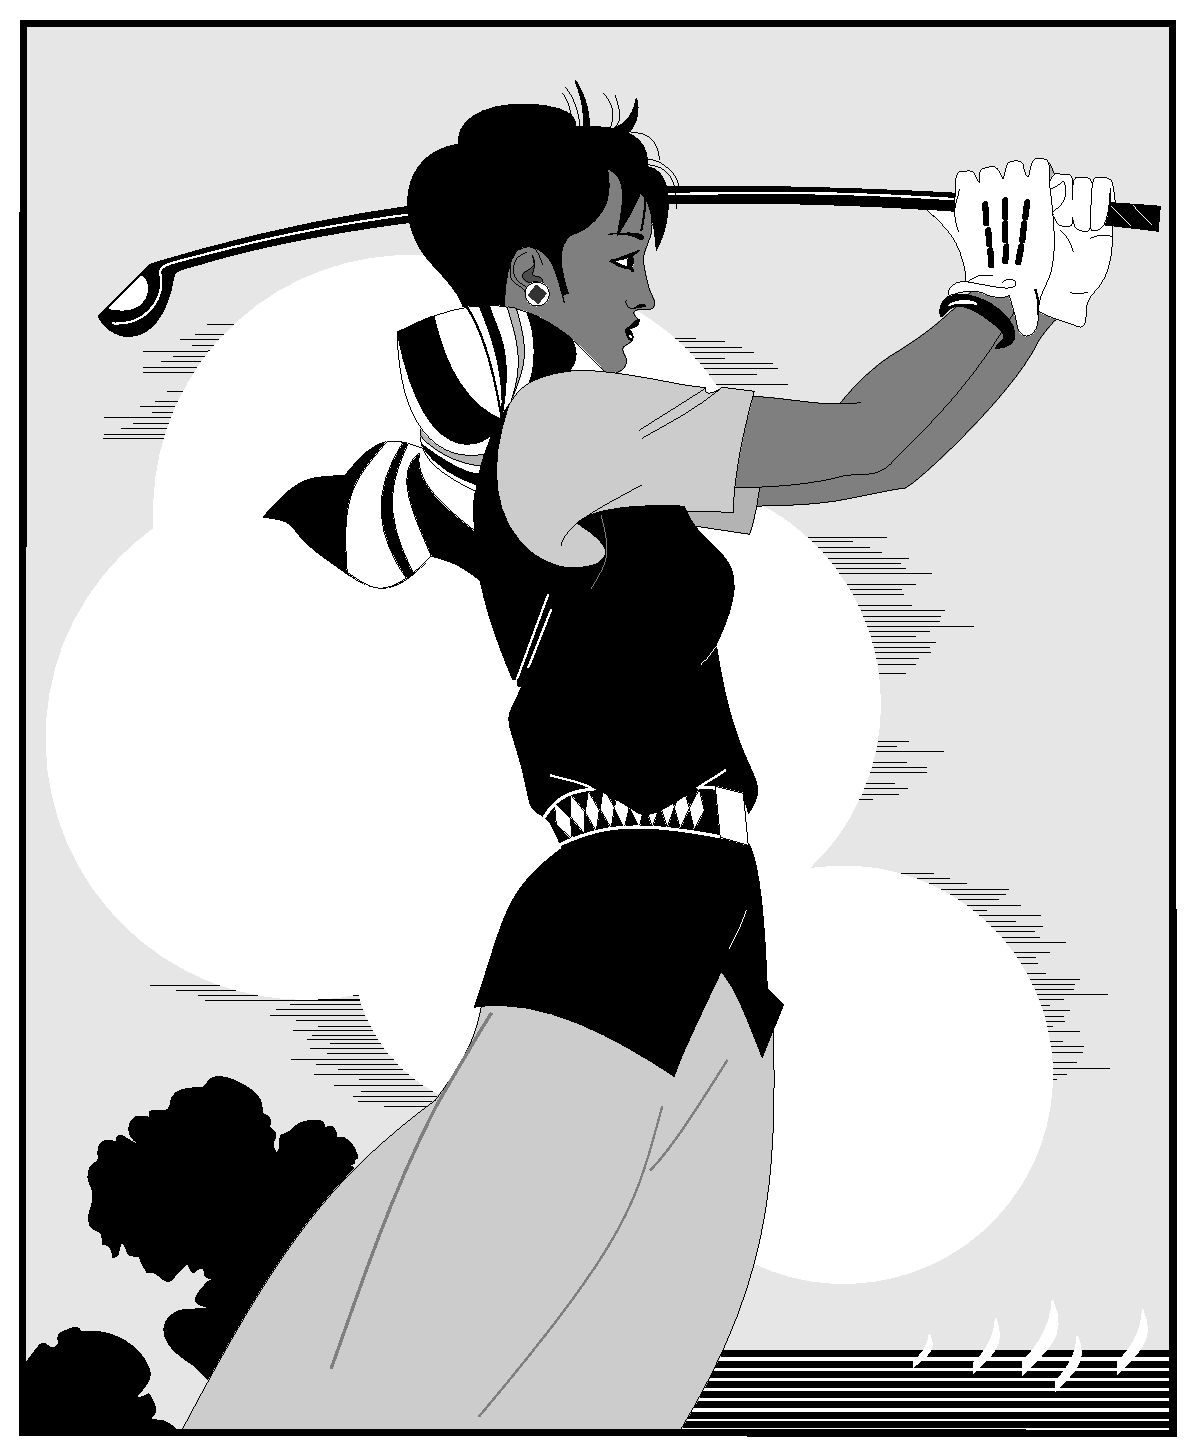
\includegraphics[width = 0.4\textwidth]{golfer}
\caption{打高尔夫球的人}
\end{figure}

\subsection{并排图和子图}[Abreast-picture and Sub-picture example]
\subsubsection{并排图}[Abreast-picture example]
\begin{figure}[htbp]
\centering
\begin{minipage}{0.4\textwidth}
\centering
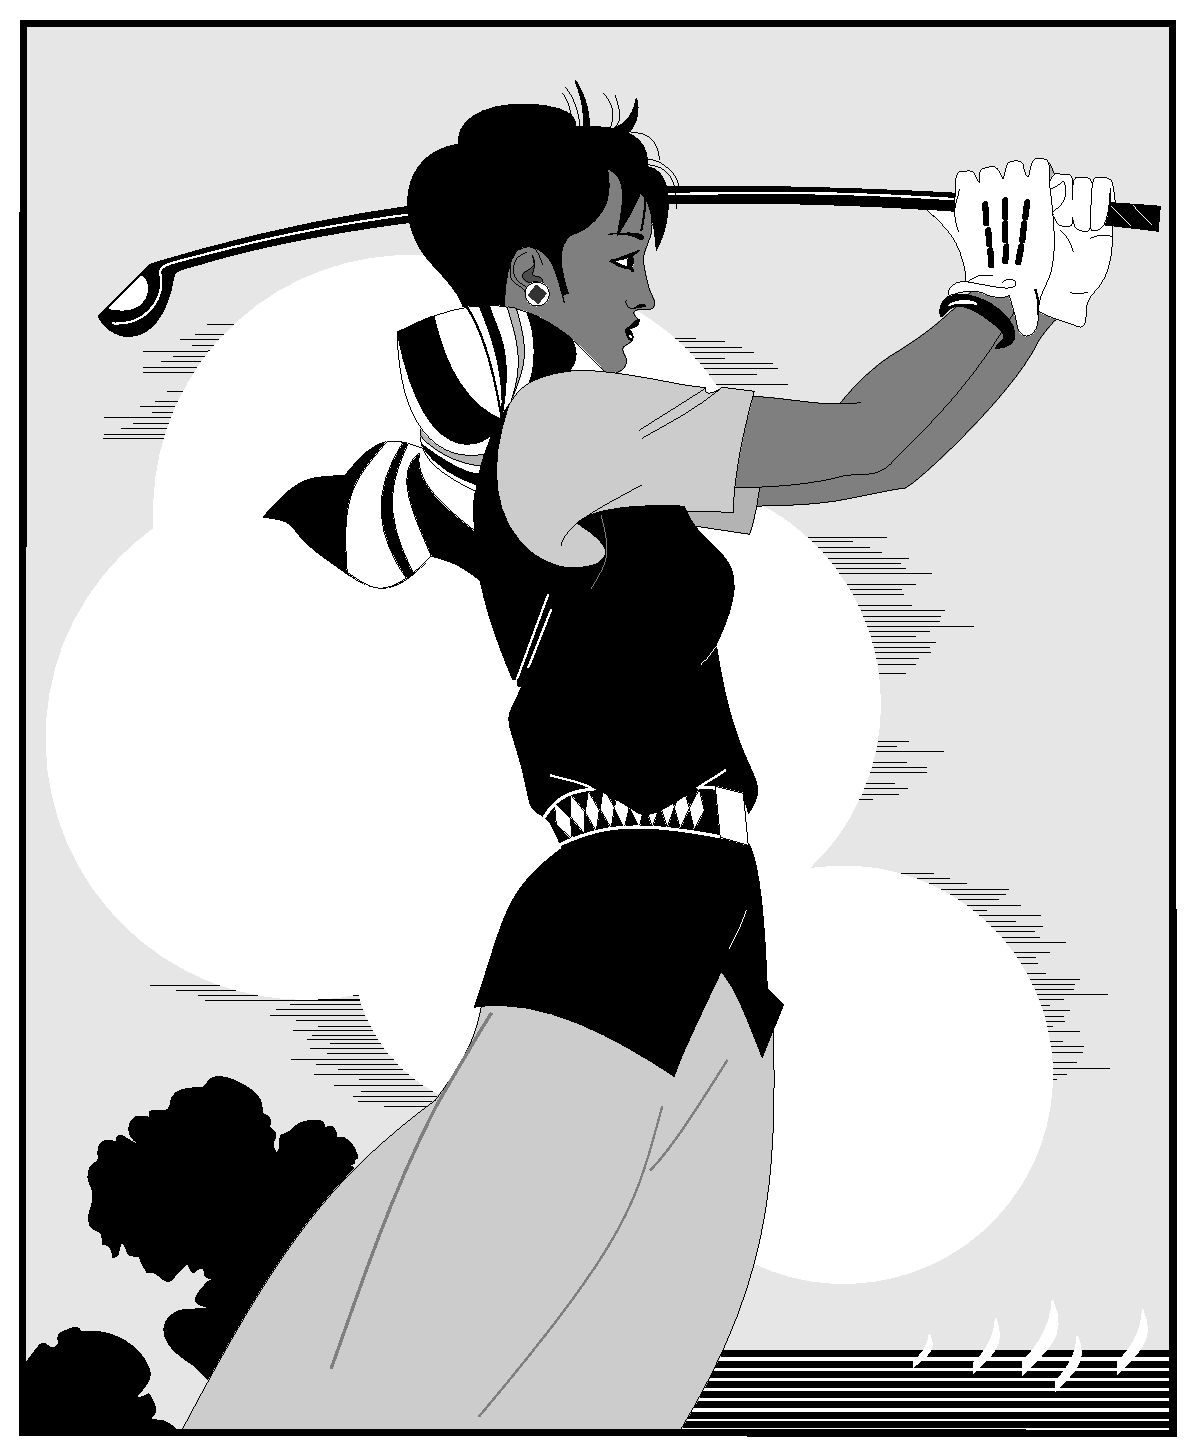
\includegraphics[width=\textwidth]{golfer}
\bicaption[golfer2]{}{打高尔夫球的人}{Fig.$\!$}{The person playing golf}
\end{minipage}
\begin{minipage}{0.4\textwidth}
\centering
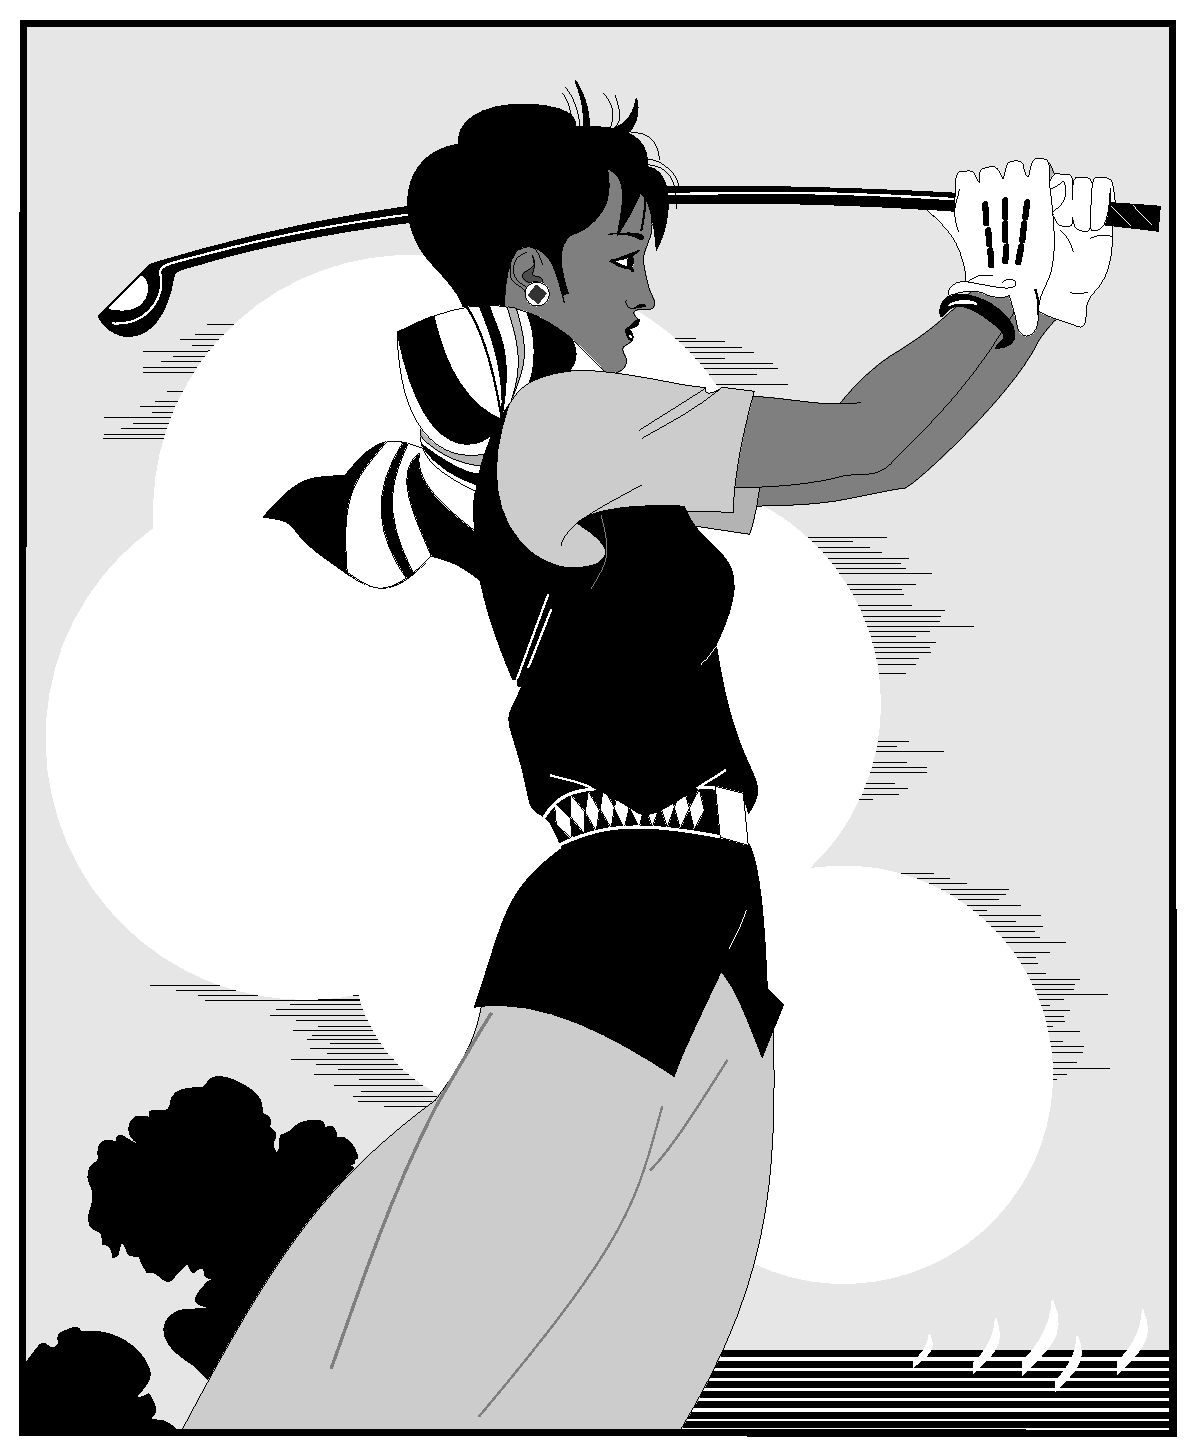
\includegraphics[width=\textwidth]{golfer}
\bicaption[golfer3]{}{打高尔夫球的人}{Fig.$\!$}{The person playing golf}
\end{minipage}
\end{figure}
\subsubsection{子图}[Sub-picture example]
注意:子图题注也可以只用中文。
\begin{figure}[!h]
\setlength{\subfigcapskip}{-1bp}
\centering
\subfigure{\label{golfer41}}\addtocounter{subfigure}{-2}
\subfigure[The person playing golf]{\subfigure[打高尔夫球的人~1]{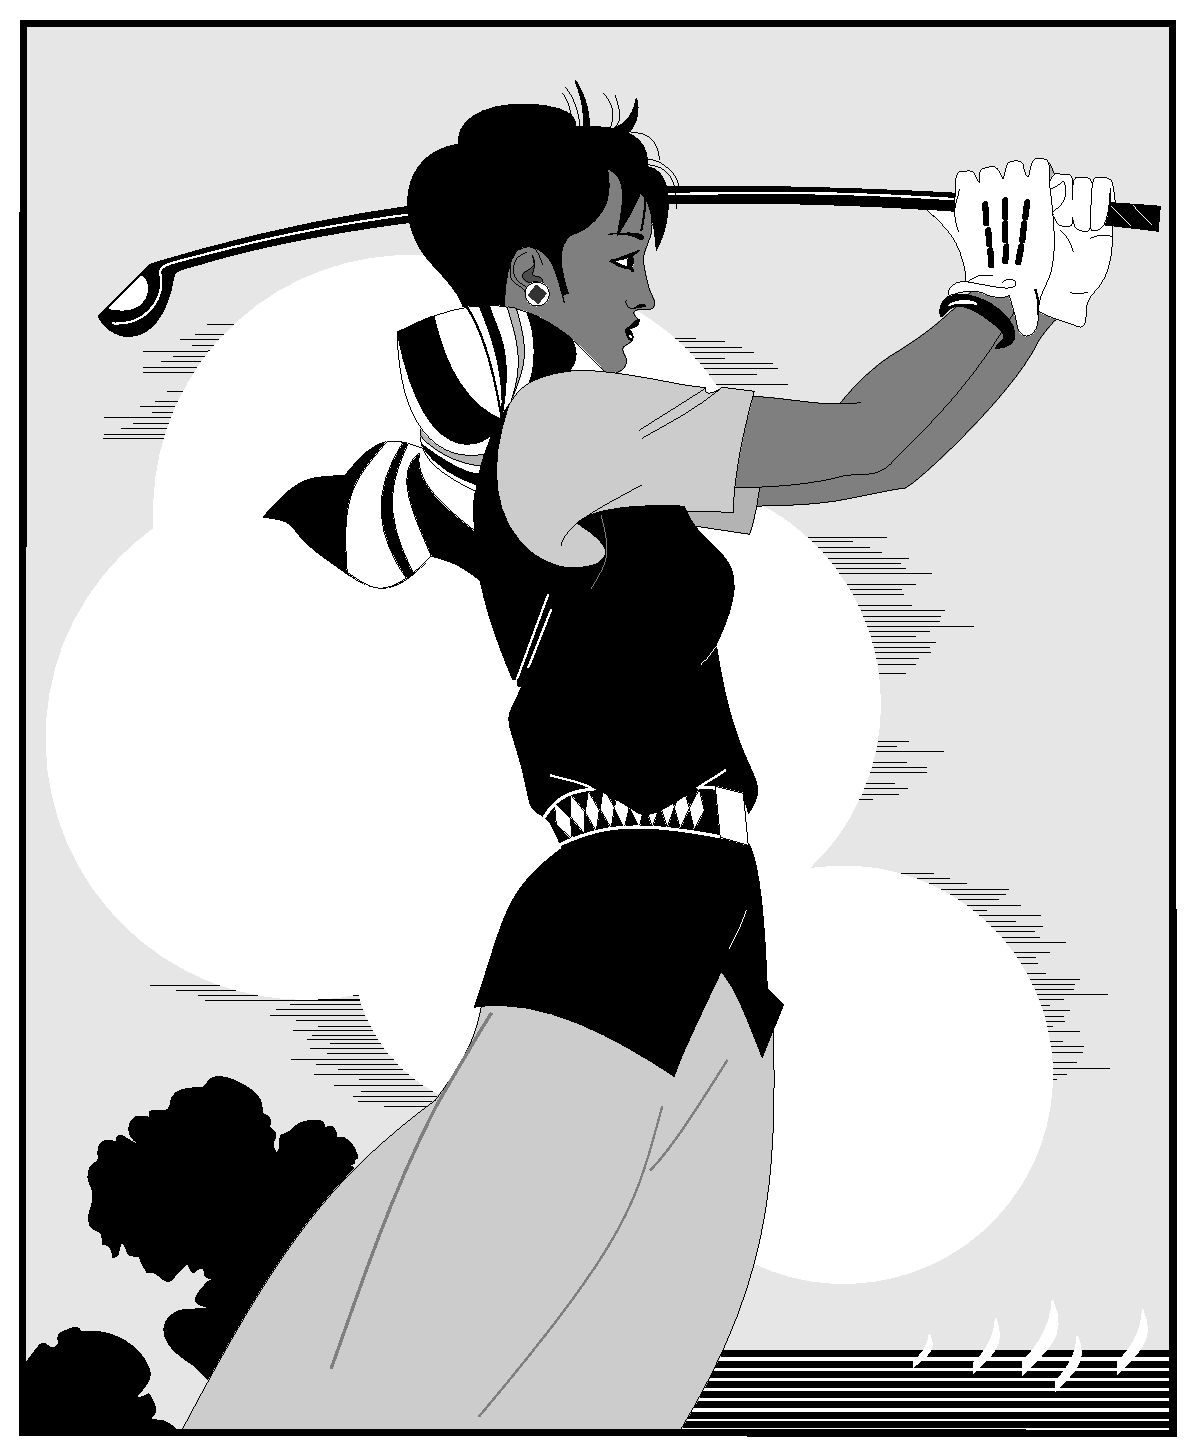
\includegraphics[width=0.4\textwidth]{golfer}}}
\subfigure{\label{golfer42}}\addtocounter{subfigure}{-2}
\subfigure[The person playing golf]{\subfigure[打高尔夫球的人~2]{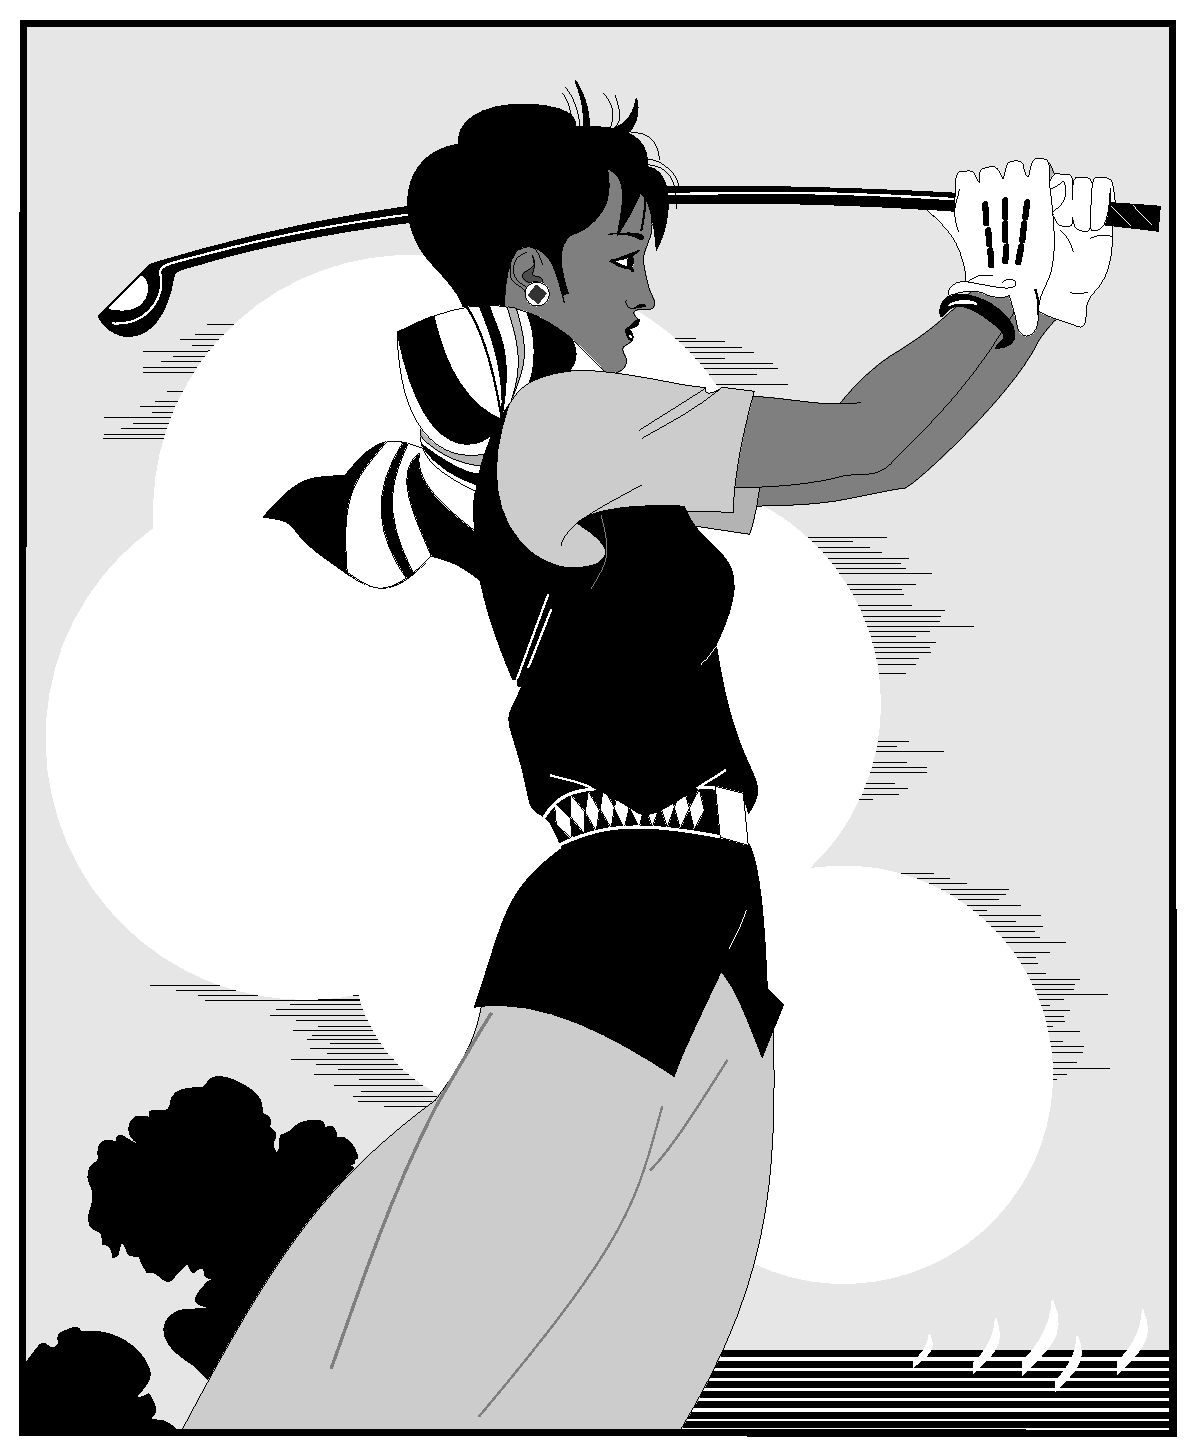
\includegraphics[width=0.4\textwidth]{golfer}}}
\subfigure{\label{golfer43}}\addtocounter{subfigure}{-2}
\subfigure[The person playing golf]{\subfigure[打高尔夫球的人~3]{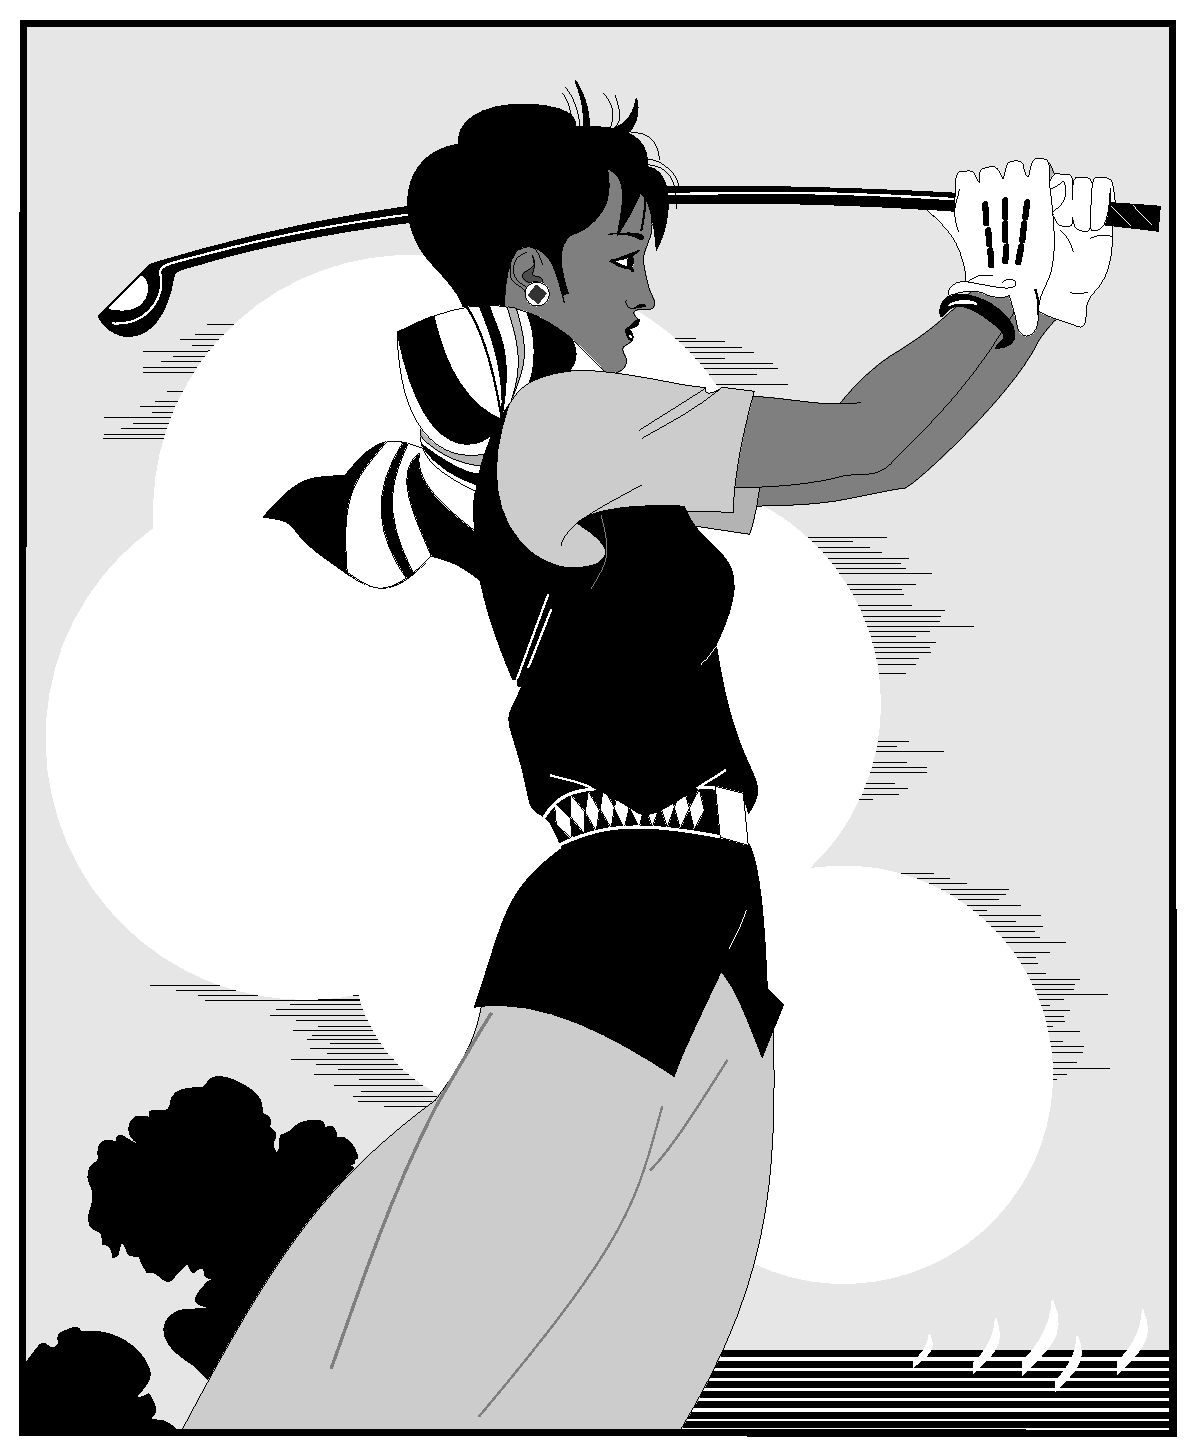
\includegraphics[width=0.4\textwidth]{golfer}}}
\subfigure{\label{golfer44}}\addtocounter{subfigure}{-2}
\subfigure[The person playing golf]{\subfigure[打高尔夫球的人~4]{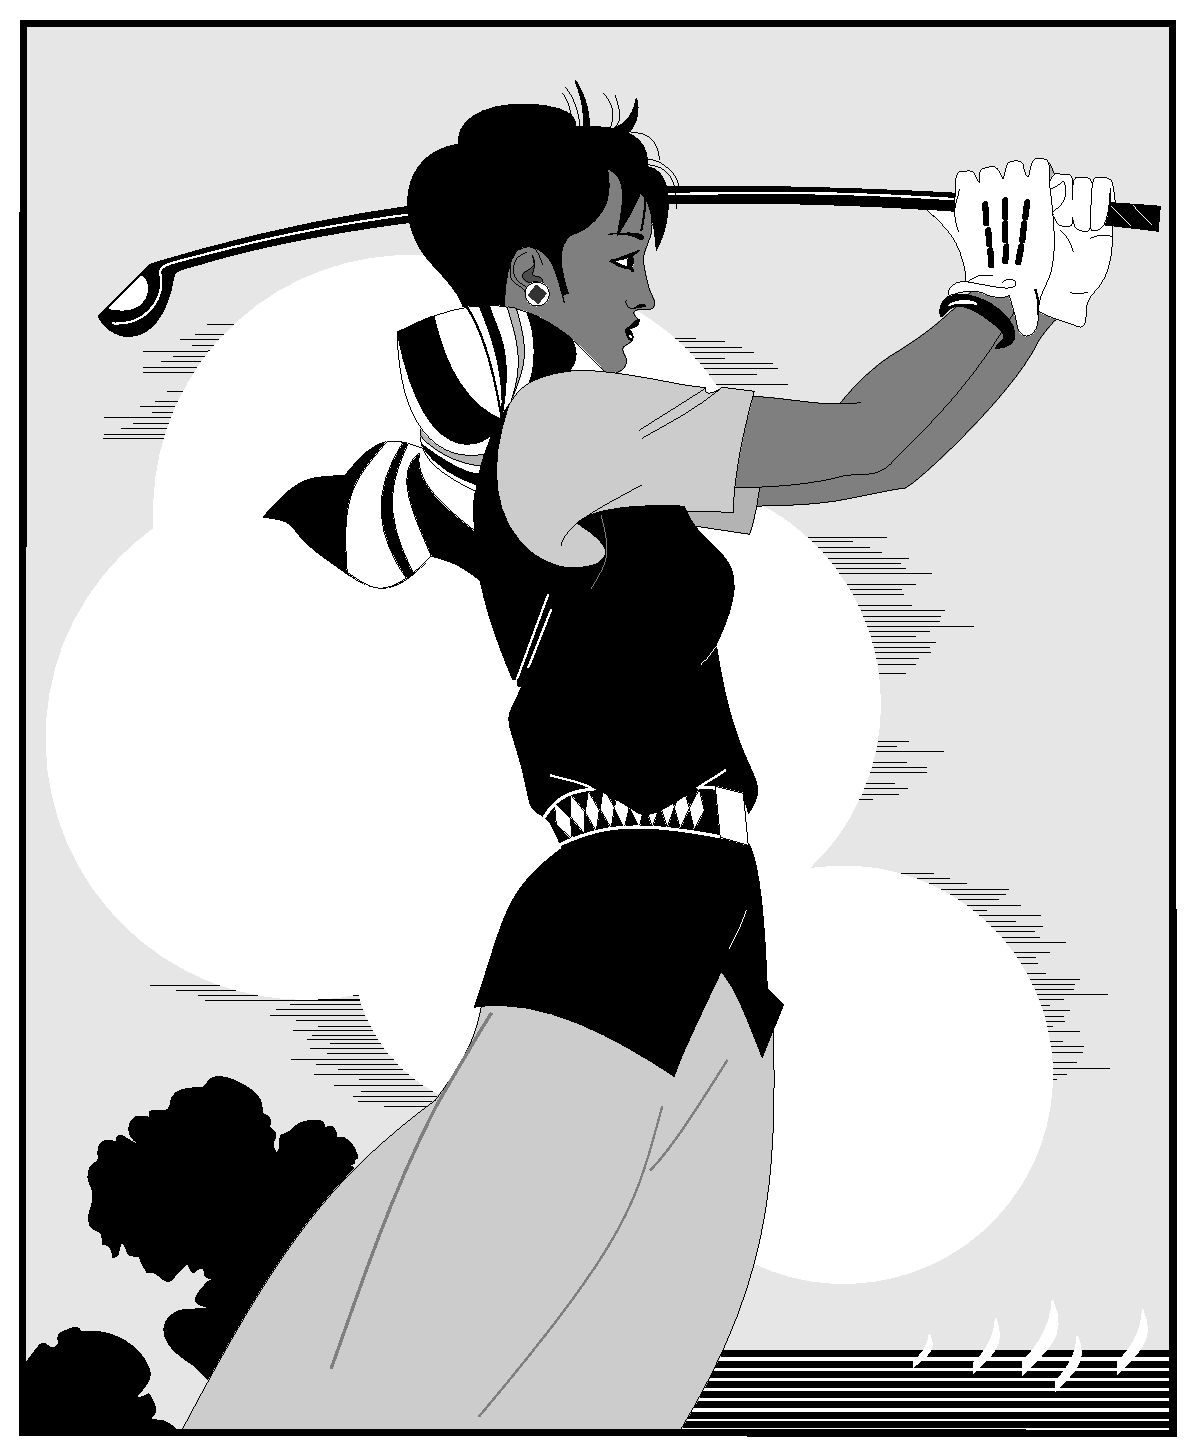
\includegraphics[width=0.4\textwidth]{golfer}}}
\vspace{0.2em}
\bicaption[golfer4]{}{打高尔夫球的人}{Fig.$\!$}{The person playing golf}
\end{figure}

\section{表格}

表应有自明性。表格不加左、右边线。表的编排建议采用国际通行的三线表。表中文字用宋
体~5~号字。每个表格均应有表题(由表序和表名组成)。表序一般按章编排,如第~1~章第
一个插表的序号为“表~1-1”等。表序与表名之间空一格,表名中不允许使用标点符号,表名
后不加标点。表题置于表上,硕士学位论文只用中文,博士学位论文用中、英文两种文字居
中排写,中文在上,要求中文用宋体~5~号字,英文用新罗马字体~5~号字。表头设计应简单
明了,尽量不用斜线。表头中可采用化学符号或物理量符号。


\subsection{普通表格的绘制方法}[Methods of drawing normal tables]

表格应具有三线表格式,因此需要调用~booktabs~宏包,其标准格式如表~\ref{table1}~所示。
\begin{table}[htbp]
\bicaption[table1]{}{符合研究生院绘图规范的表格}{Table$\!$}{Table in agreement of the standard from graduate school}
\vspace{0.5em}\centering\wuhao
\begin{tabular}{ccccc}
\toprule[1.5pt]
$D$(in) & $P_u$(lbs) & $u_u$(in) & $\beta$ & $G_f$(psi.in)\\
\midrule[1pt]
 5 & 269.8 & 0.000674 & 1.79 & 0.04089\\
10 & 421.0 & 0.001035 & 3.59 & 0.04089\\
20 & 640.2 & 0.001565 & 7.18 & 0.04089\\
\bottomrule[1.5pt]
\end{tabular}
\end{table}
全表如用同一单位,则将单位符号移至表头右上角,加圆括号。表中数据应准确无误,书写
清楚。数字空缺的格内加横线“-”(占~2~个数字宽度)。表内文字或数字上、下或左、右
相同时,采用通栏处理方式,不允许用“〃”、“同上”之类的写法。表内文字说明,起行空一
格、转行顶格、句末不加标点。如某个表需要转页接排,在随后的各页上应重复表的编号。
编号后加“(续表)”,表题可省略。续表应重复表头。

\subsection{长表格的绘制方法}[Methods of drawing long tables]

长表格是当表格在当前页排不下而需要转页接排的情况下所采用的一种表格环境。若长表格
仍按照普通表格的绘制方法来获得,其所使用的\verb|table|浮动环境无法实现表格的换页
接排功能,表格下方过长部分会排在表格第1页的页脚以下。为了能够实现长表格的转页接
排功能,需要调用~longtable~宏包,由于长表格是跨页的文本内容,因此只需要单独的
\verb|longtable|环境,所绘制的长表格的格式如表~\ref{table2}~所示。

注意,长表格双语标题的格式。

\ltfontsize{\dawu[1.667]}
\dawu[1.667]\begin{longtable}{ccc}%
\longbionenumcaption{}{{\wuhao 中国省级行政单位一览
}\label{table2}}{Table$\!$}{}{{\wuhao Overview of the provincial administrative
unit of China}}{-0.5em}{3.15bp}\\
%\caption{\wuhao 中国省级行政单位一览}\\
\toprule[1.5pt] 名称 & 简称 & 省会或首府  \\ \midrule[1pt]
\endfirsthead
\multicolumn{3}{r}{表~\thetable(续表)}\vspace{0.5em}\\
\toprule[1.5pt] 名称 & 简称 & 省会或首府  \\ \midrule[1pt]
\endhead
\bottomrule[1.5pt]
\endfoot
北京市 & 京 & 北京\\
天津市 & 津 & 天津\\
河北省 & 冀 & 石家庄市\\
山西省 & 晋 & 太原市\\
内蒙古自治区 & 蒙 & 呼和浩特市\\
辽宁省 & 辽 & 沈阳市\\
吉林省 & 吉 & 长春市\\
黑龙江省 & 黑 & 哈尔滨市\\
上海市 & 沪/申 & 上海\\
江苏省 & 苏 & 南京市\\
浙江省 & 浙 & 杭州市\\
安徽省 & 皖 & 合肥市\\
福建省 & 闽 & 福州市\\
江西省 & 赣 & 南昌市\\
山东省 & 鲁 & 济南市\\
河南省 & 豫 & 郑州市\\
湖北省 & 鄂 & 武汉市\\
湖南省 & 湘 & 长沙市\\
广东省 & 粤 & 广州市\\
广西壮族自治区 & 桂 & 南宁市\\
海南省 & 琼 & 海口市\\
重庆市 & 渝 & 重庆\\
四川省 & 川/蜀 & 成都市\\
贵州省 & 黔/贵 & 贵阳市\\
云南省 & 云/滇 & 昆明市\\
西藏自治区 & 藏 & 拉萨市\\
陕西省 & 陕/秦 & 西安市\\
甘肃省 & 甘/陇 & 兰州市\\
青海省 & 青 & 西宁市\\
宁夏回族自治区 & 宁 & 银川市\\
新疆维吾尔自治区 & 新 & 乌鲁木齐市\\
香港特别行政区 & 港 & 香港\\
澳门特别行政区 & 澳 & 澳门\\
台湾省 & 台 & 台北市\\
\end{longtable}\normalsize

\ltfontsize{\dawu[1.667]}
\dawu[1.667]\begin{longtable}{ccc}%
  \caption{\wuhao 中国省级行政单位一览}\\[0.3em]
\toprule[1.5pt] 名称 & 简称 & 省会或首府  \\ \midrule[1pt]
\endfirsthead
\multicolumn{3}{r}{表~\thetable(续表)}\vspace{0.5em}\\
\toprule[1.5pt] 名称 & 简称 & 省会或首府  \\ \midrule[1pt]
\endhead
\bottomrule[1.5pt]
\endfoot
北京市 & 京 & 北京\\
天津市 & 津 & 天津\\
河北省 & 冀 & 石家庄市\\
山西省 & 晋 & 太原市\\
内蒙古自治区 & 蒙 & 呼和浩特市\\
辽宁省 & 辽 & 沈阳市\\
吉林省 & 吉 & 长春市\\
黑龙江省 & 黑 & 哈尔滨市\\
上海市 & 沪/申 & 上海\\
江苏省 & 苏 & 南京市\\
浙江省 & 浙 & 杭州市\\
安徽省 & 皖 & 合肥市\\
福建省 & 闽 & 福州市\\
江西省 & 赣 & 南昌市\\
山东省 & 鲁 & 济南市\\
河南省 & 豫 & 郑州市\\
湖北省 & 鄂 & 武汉市\\
湖南省 & 湘 & 长沙市\\
广东省 & 粤 & 广州市\\
广西壮族自治区 & 桂 & 南宁市\\
海南省 & 琼 & 海口市\\
重庆市 & 渝 & 重庆\\
四川省 & 川/蜀 & 成都市\\
贵州省 & 黔/贵 & 贵阳市\\
云南省 & 云/滇 & 昆明市\\
西藏自治区 & 藏 & 拉萨市\\
陕西省 & 陕/秦 & 西安市\\
甘肃省 & 甘/陇 & 兰州市\\
青海省 & 青 & 西宁市\\
宁夏回族自治区 & 宁 & 银川市\\
新疆维吾尔自治区 & 新 & 乌鲁木齐市\\
香港特别行政区 & 港 & 香港\\
澳门特别行政区 & 澳 & 澳门\\
台湾省 & 台 & 台北市\\
\end{longtable}\normalsize
此长表格~\ref{table2}~第~2~页的标题“编号(续表)”和表头是通过代码自动添加上去的,无需人工添加,若表格在页面中的竖直位置发生了变化,长表格在第~2~页
及之后各页的标题和表头位置能够始终处于各页的最顶部,也无需人工调整,\LaTeX~系统的这一优点是~word~等软件所无法比拟的。

\subsection{列宽可调表格的绘制方法}[Methods of drawing tables with adjustable-width columns]
论文中能用到列宽可调表格的情况共有两种,一种是当插入的表格某一单元格内容过长以至
于一行放不下的情况,另一种是当对公式中首次出现的物理量符号进行注释的情况,这两种
情况都需要调用~tabularx~宏包。下面将分别对这两种情况下可调表格的绘制方法进行阐述
。
\subsubsection{表格内某单元格内容过长的情况}[The condition when the contents in
some cells of tables are too long]
首先给出这种情况下的一个例子如表~\ref{table3}~所示。
\begin{table}[htbp]
  \centering
\bicaption[table3]{}{最小的三个正整数的英文表示法}{Table$\!$}{The English construction of the smallest three positive integral numbers}\vspace{0.5em}\wuhao
\begin{tabularx}{0.7\textwidth}{llX}
\toprule[1.5pt]
Value & Name & Alternate names, and names for sets of the given size\\\midrule[1pt]
1 & One & ace, single, singleton, unary, unit, unity\\
2 & Two & binary, brace, couple, couplet, distich, deuce, double, doubleton, duad, duality, duet, duo, dyad, pair, snake eyes, span, twain, twosome, yoke\\
3 & Three & deuce-ace, leash, set, tercet, ternary, ternion, terzetto, threesome, tierce, trey, triad, trine, trinity, trio, triplet, troika, hat-trick\\\bottomrule[1.5pt]
\end{tabularx}
\end{table}
tabularx环境共有两个必选参数:第1个参数用来确定表格的总宽度,第2个参数用来确定每
列格式,其中标为X的项表示该列的宽度可调,其宽度值由表格总宽度确定。标为X的列一般
选为单元格内容过长而无法置于一行的列,这样使得该列内容能够根据表格总宽度自动分行
。若列格式中存在不止一个X项,则这些标为X的列的列宽相同,因此,一般不将内容较短的
列设为X。标为X的列均为左对齐,因此其余列一般选为l(左对齐),这样可使得表格美观
,但也可以选为c或r。

\subsubsection{对物理量符号进行注释的情况}[The condition when physical symbols
need to be annotated]

为使得对公式中物理量符号注释的转行与破折号“———”后第一个字对齐,此处最好采用表格
环境。此表格无任何线条,左对齐,且在破折号处对齐,一共有“式中”二字、物理量符号和
注释三列,表格的总宽度可选为文本宽度,因此应该采用\verb|tabularx|环境。由
\verb|tabularx|环境生成的对公式中物理量符号进行注释的公式如式(\ref{eq:1})所示。
\begin{equation}\label{eq:1}
\ddot{\boldsymbol{\rho}}-\frac{\mu}{R_{t}^{3}}\left(3\mathbf{R_{t}}\frac{\mathbf{R_{t}\rho}}{R_{t}^{2}}-\boldsymbol{\rho}\right)=\mathbf{a}
\end{equation}
\begin{tabularx}{\textwidth}{@{}l@{\quad}r@{———}X@{}}
式中& $\boldsymbol{\rho}$ &追踪飞行器与目标飞行器之间的相对位置矢量;\\
&  $\boldsymbol{\ddot{\rho}}$&追踪飞行器与目标飞行器之间的相对加速度;\\
&  $\mathbf{a}$   &推力所产生的加速度;\\
&  $\mathbf{R_t}$ & 目标飞行器在惯性坐标系中的位置矢量;\\
&  $\omega_{t}$ & 目标飞行器的轨道角速度;\\
&  $\mathbf{g}$ & 重力加速度,$=\frac{\mu}{R_{t}^{3}}\left(
3\mathbf{R_{t}}\frac{\mathbf{R_{t}\rho}}{R_{t}^{2}}-\boldsymbol{\rho}\right)=\omega_{t}^{2}\frac{R_{t}}{p}\left(
3\mathbf{R_{t}}\frac{\mathbf{R_{t}\rho}}{R_{t}^{2}}-\boldsymbol{\rho}\right)$,这里~$p$~是目标飞行器的轨道半通径。
\end{tabularx}\vspace{3.15bp}
由此方法生成的注释内容应紧邻待注释公式并置于其下方,因此不能将代码放入
\verb|table|浮动环境中。但此方法不能实现自动转页接排,可能会在当前页剩余空间不够
时,全部移动到下一页而导致当前页出现很大空白。因此在需要转页处理时,还请您手动将
需要转页的代码放入一个新的\verb|tabularx|环境中,将原来的一个\verb|tabularx|环境
拆分为两个\verb|tabularx|环境。

\section{公式}
与正常\LaTeX\ 使用方法一致,此处略。关于公式中符号样式的定义在`hithesis.sty'有示
例。

\section{其他杂项}[Miscellaneous]

\subsection{算法}[Algorithms]
我工算法有以下几大特点。

(1)算法不再规范中要求。

(2)算法常常被使用(至少计算机学院)。

(3)格式乱,甚至出现了每个实验室的格式要求都不一样。

此处不给出示例,因为没法给,在
\href{https://github.com/dustincys/PlutoThesis}{https://github.com/dustincys/PlutoThesis}
的readme文件中有不同实验室算法要求说明。

\subsection{脚注}[Footnotes]
不再规范\footnote{规范是指\PGR\ 和\UGR}中要求,模板默认使用清华大学的格式。

\subsection{源码}[Source code]
也不再规范中要求。如果有需要最好使用minted包,但在编译的时候需要添加“
-shell-escape”选项且安装pygmentize软件,这些不在模板中默认载入,如果需要自行载入
。
\subsection{思源宋体}[Siyuan font]
如果要使用思源字体,需要思源字体的定义文件,此文件请到模板的开发版网址github:
\href{https://gihitb.com/dustincys/hithesis}{https://gihitb.com/dustincys/hithesis}
或者oschia:
\href{https://git.oschina.net/dustincys/hithesis}{https://git.oschina.net/dustincys/hithesis}
处下载。

\subsection{专业绘图工具}[Processional drawing tool]
推荐使用tikz包,使用tikz源码绘图的好处是,图片中的字体与正文中的字体一致。具体如
何使用tikz绘图不属于模板范畴。
tikz适合用来画不需要大量实验数据支撑示意图。但R语言等专业绘图工具具有画出各种、
专业、复杂的数据图。R语言中有tikz包,能自动生成tikz码,这样tikz几乎无所不能。
对于排版有极致追求的小伙伴,可以参考
\href{http://www.texample.net/tikz/resources/}{http://www.texample.net/tikz/resources/}
中所列工具,几乎所有作图软件所作的图形都可一转成tikz,然后可以自由的在tikz中修改
图中内容,定义字体等等。实现前文窝工规范中要求的图中字体的一致性的终极目标。


\subsection{术语词汇管理}[Manage glossaries]
推荐使用glossaries包管理术语、缩略语,可以自动生成首次全写,非首次缩写。

\subsection{\TeX\ 源码编辑器}[\TeX editor]
推荐:(1)付费软件Winedt;(2)免费软件kile;(3)vim或emaces或sublime等神级编
译器(需要配置)。

\subsection{\LaTeX\ 排版重要原则}[\LaTeX\ typesetting rules]
格式和内容分离是\LaTeX\ 最大优势,所有多次出现的内容、样式等等都可以定义为简单命
令、环境。这样的好处是方便修改、管理。例如,如果想要把所有的表示向量的符号由粗体
\cs{mathbf}变换到花体\cs{mathcal},只需修改该格式的命令的定义部分,不需要像MS
word那样处处修改。总而言之,使用自定义命令和环境才是正确的使用\LaTeX\ 的方式。

\section{关于捐助}
各位刀客和大侠如用的嗨,要解囊相助,请微信或支付宝参照图
~\ref{wct5}~到图~\ref{zfb}~中提示操作(二维码被矢量化后之后去
除了头像等冗余无用的部分~)。

\begin{figure}[!h]
\setlength{\subfigcapskip}{-1bp}
\centering
\subfigure{\label{wct5}}\addtocounter{subfigure}{-1}
\subfigure[如果用的嗨,微信扫码捐助5元~~]{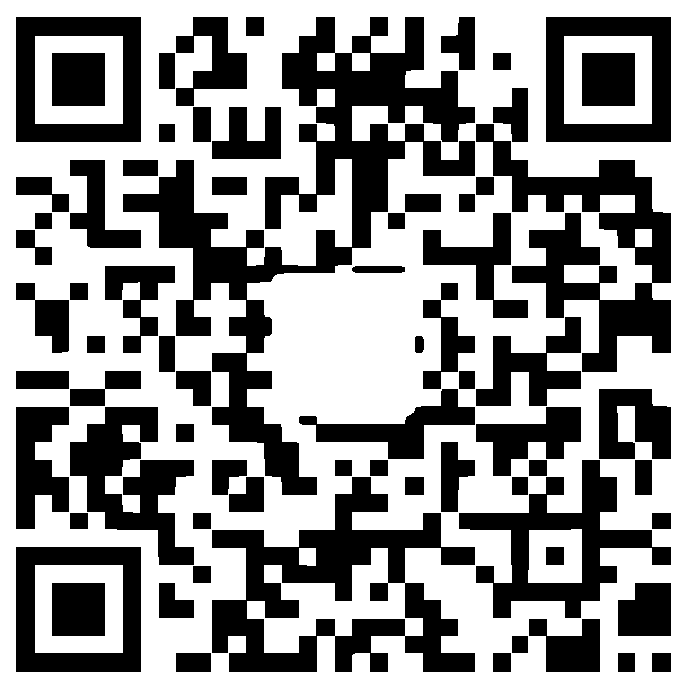
\includegraphics[width=0.4\textwidth]{wct5}}
\hspace{2em}
\subfigure{\label{wct10}}\addtocounter{subfigure}{-1}
\subfigure[如果用的非常嗨,微信扫码捐助10元~~]{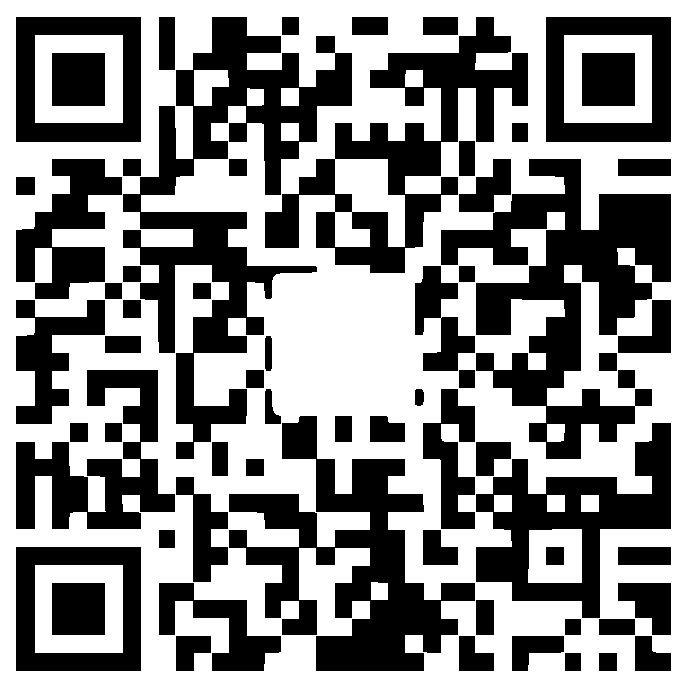
\includegraphics[width=0.4\textwidth]{wct10}}
\subfigure{\label{wct1}}\addtocounter{subfigure}{-1}
\subfigure[那个,看在熬夜写代码的份上,微信扫码捐助1元吧~~]{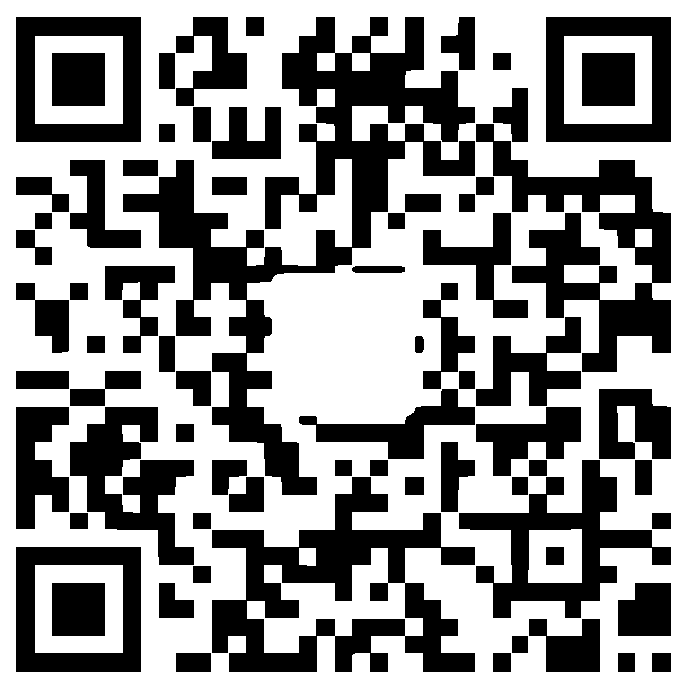
\includegraphics[width=0.4\textwidth]{wct1}}
\hspace{2em}
\subfigure{\label{zfb}}\addtocounter{subfigure}{-1}
\subfigure[或者支付宝不限额度~]{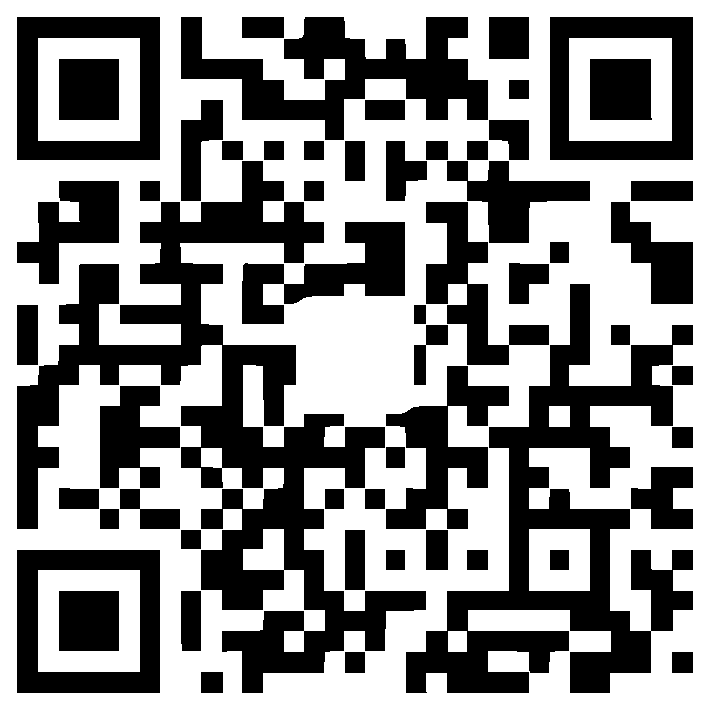
\includegraphics[width=0.4\textwidth]{zfb}}
\vspace{0.2em}
\bicaption[Donation]{}{捐助,注意此处是子图只用汉语图题的形式,我工规定可以不用
英语图题}{Fig.$\!$}{Donation, please note that it is OK to use Chinese caption
only}
\end{figure}


%======================================================================
\backmatter
%硕博书序
% !Mode:: "TeX:UTF-8" 
\begin{conclusions}

学位论文的结论作为论文正文的最后一章单独排写,但不加章标题序号。

结论应是作者在学位论文研究过程中所取得的创新性成果的概要总结,不能与摘要混为一谈。博士学位论文结论应包括论文的主要结果、创新点、展望三部分,在结论中应概括论文的核心观点,明确、客观地指出本研究内容的创新性成果(含新见解、新观点、方法创新、技术创新、理论创新),并指出今后进一步在本研究方向进行研究工作的展望与设想。对所取得的创新性成果应注意从定性和定量两方面给出科学、准确的评价,分(1)、(2)、(3)…条列出,宜用“提出了”、“建立了”等词叙述。

\end{conclusions}
   % 结论
\bibliographystyle{hithesis} %如果没有参考文献时候
\bibliography{reference}
%\begin{appendix}%附录
%% -*-coding: utf-8 -*-
%%%%%%%%%%%%%%%%%%%%%%%%%%%%%%%%%%%%%%%%%%%%%%%%%%%%%%%%%
\chapter{带章节的附录}[Full Appendix]%
完整的附录内容,包含章节,公式,图表等

%%%%%%%%%%%%%%%%%%%%%%%%%%%%%%%%%%%%%%%%%%%%%%%%%%%%%%%%%
\section{附录节的内容}[Section in Appendix]
这是附录的节的内容

附录中图的示例:
\begin{figure}[htbp]
\centering
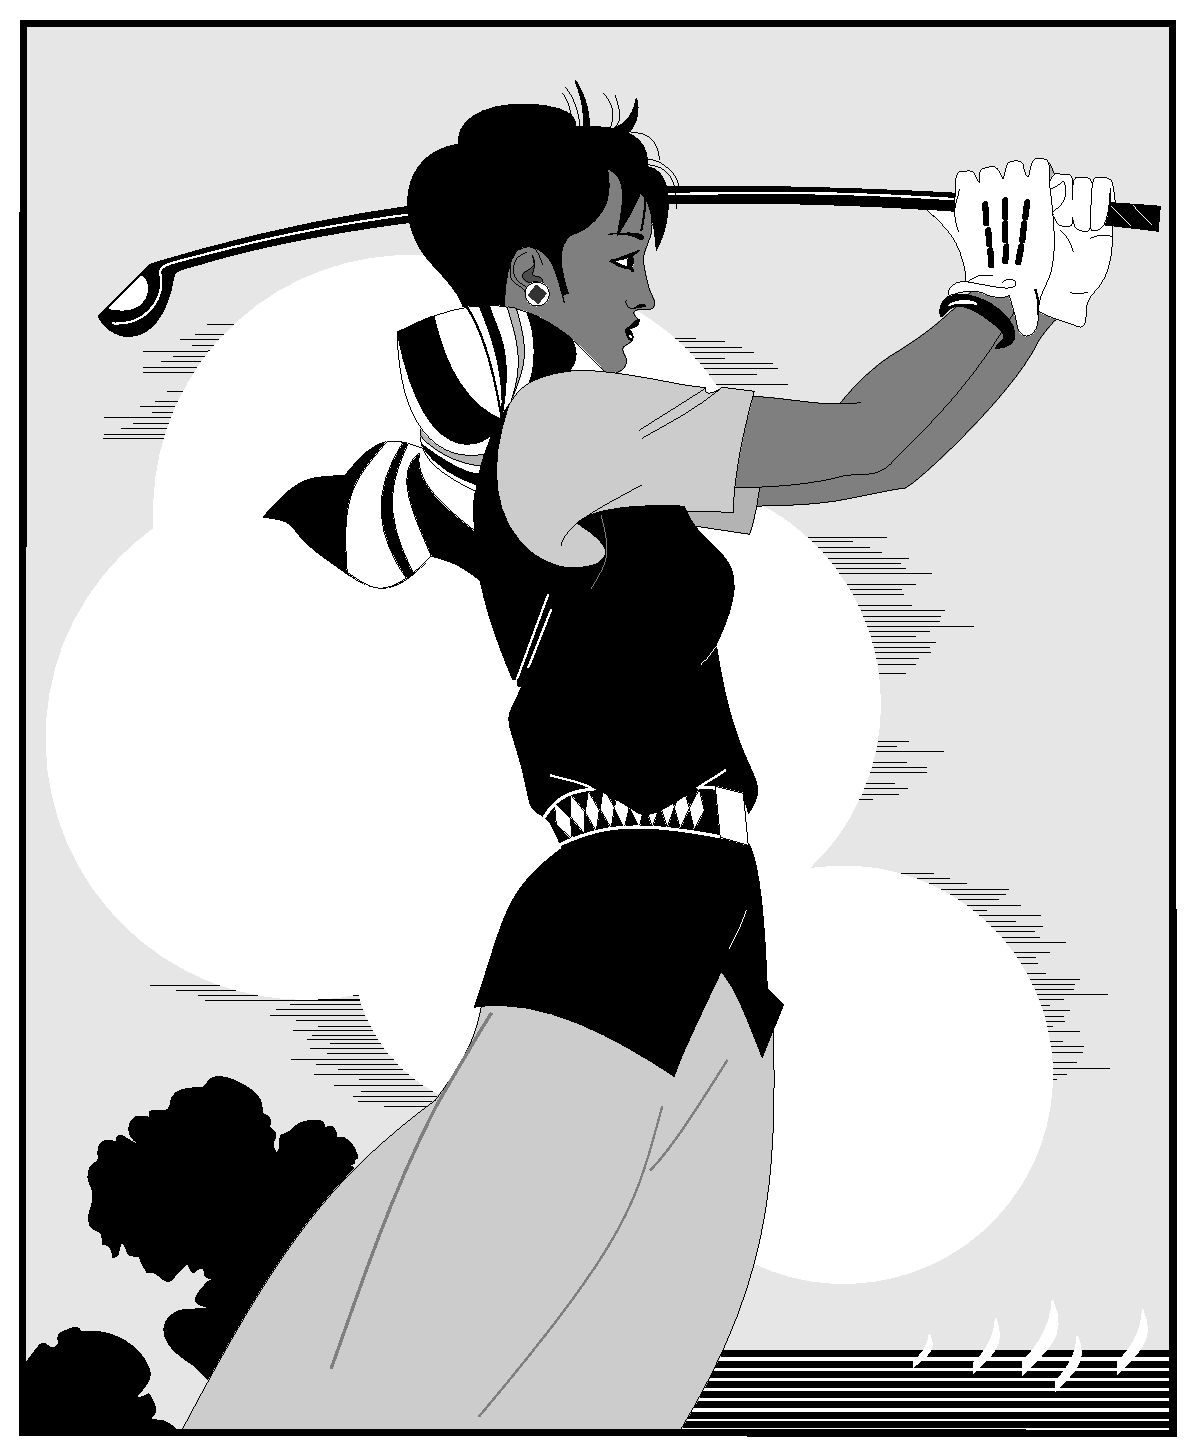
\includegraphics[width = 0.4\textwidth]{golfer}
%\bicaption[golfer5]{}{\xiaosi[0]打高尔夫球的人}{Fig.$\!$}{The person playing golf}\vspace{-1em}
\caption{\xiaosi[0]打高尔夫球的人}
\end{figure}

附录中公式的示例:
\begin{align}
a & = b \times c \\
E & = m c^2
\label{eq}
\end{align}

\chapter{这个星球上最好的免费Linux软件列表}[List of the Best Linux Software in our Planet]
\section*{系统}

\href{http://fvwm.org/}{FVWM 星球最强大的窗口管理器}——推荐

\section*{其他}

\href{https://github.com/goldendict/goldendict}{goldendict 星球最强大的桌面字典}——推荐

\href{http://www.mutt.org/}{mutt 星球最强大的邮件客户端}——推荐

%\end{appendix}
% !Mode:: "TeX:UTF-8" 

\begin{publication}
\noindent\textbf{(一)发表的学术论文}
\begin{publist}
\item	XXX,XXX. Static Oxidation Model of Al-Mg/C Dissipation Thermal Protection Materials[J]. Rare Metal Materials and Engineering, 2010, 39(Suppl. 1): 520-524.(SCI~收录,IDS号为~669JS,IF=0.16)
\item XXX,XXX. 精密超声振动切削单晶铜的计算机仿真研究[J]. 系统仿真学报,2007,19(4):738-741,753.(EI~收录号:20071310514841)
\item XXX,XXX. 局部多孔质气体静压轴向轴承静态特性的数值求解[J]. 摩擦学学报,2007(1):68-72.(EI~收录号:20071510544816)
\item XXX,XXX. 硬脆光学晶体材料超精密切削理论研究综述[J]. 机械工程学报,2003,39(8):15-22.(EI~收录号:2004088028875)
\item XXX,XXX. 基于遗传算法的超精密切削加工表面粗糙度预测模型的参数辨识以及切削参数优化[J]. 机械工程学报,2005,41(11):158-162.(EI~收录号:2006039650087)
\item XXX,XXX. Discrete Sliding Mode Cintrok with Fuzzy Adaptive Reaching Law on 6-PEES Parallel Robot[C]. Intelligent System Design and Applications, Jinan, 2006: 649-652.(EI~收录号:20073210746529)
\end{publist}

\noindent\textbf{(二)申请及已获得的专利(无专利时此项不必列出)}
\begin{publist}
\item XXX,XXX. 一种温热外敷药制备方案:中国,88105607.3[P]. 1989-07-26.
\end{publist}

\noindent\textbf{(三)参与的科研项目及获奖情况}
\begin{publist}
\item	XXX,XXX. XX~气体静压轴承技术研究, XX~省自然科学基金项目.课题编号:XXXX.
\item XXX,XXX. XX~静载下预应力混凝土房屋结构设计统一理论. 黑江省科学技术二等奖, 2007.
\end{publist}
%\vfill
%\hangafter=1\hangindent=2em\noindent
%\setlength{\parindent}{2em}
\end{publication}
    % 所发文章
%\begin{ceindex}
  %如果想要手动加索引,注释掉以下这一样,用wordlist环境
\printsubindex*
\end{ceindex}
    % 索引, 根据自己的情况添加或者不添加,选择自动添加或者手工添加。
%=======================================================================
%% 以下有需要留下,没有需要不加
% 插图索引
\listoffigures
% 表格索引
\listoftables
% 公式索引
%\listofequations
%======================================================================
\authorization %授权
%\authorization[saomiao.pdf] %添加扫描页的命令,与上互斥
% !Mode:: "TeX:UTF-8"
\begin{acknowledgements}
衷心感谢导师~XXX~教授对本人的精心指导。他的言传身教将使我终生受益。

……

感谢哈工大\LaTeX\ 论文模板\hithesis\ !

\end{acknowledgements}
 %致谢
%% !Mode:: "TeX:UTF-8" 

\begin{resume}
XXXX~年~XX~月~XX~日出生于~XXXX。

XXXX~年~XX~月考入~XX~大学~XX~院(系)XX~专业,XXXX~年~XX~月本科毕业并获得~XX~学学士学位。

XXXX~年~XX~月------XXXX~年~XX~月在~XX~大学~XX~院(系)XX~学科学习并获得~XX~学硕士学位。

XXXX~年~XX~月------XXXX~年~XX~月在~XX~大学~XX~院(系)XX~学科学习并获得~XX~学博士学位。

获奖情况:如获三好学生、优秀团干部、X~奖学金等(不含科研学术获奖)。

工作经历:

\textbf{( 除全日制硕士生以外,其余学生均应增列此项。个人简历一般应包含教育经历和工作经历。)}
\end{resume}
          % 博士学位论文有个人简介

\end{document}
 







